
\chapter{A Mapping from Role-Based Models to Context Description Logics}
\label{cha:mapping}

In the last chapter we introduced a family of description logics which are capable of expressing
contextualised knowledge. This provides the needed expressiveness to be able to reason on role-based
models. But due to the rather elaborate semantics both of role-based models and of contextualised
description logics it will be tedious and error-prone to construct the DL ontology which exactly
captures a role-based model. Hence, an automated mapping from role-based models into DL would be
desirable. Therefore, a formal representation of role-based systems with a well-defined semantics is
necessary.

In this chapter we will present a mapping from such role-based models into contextualised DLs in
order to automate this step.
%
To avoid the confusion with the notations, from now on we differentiate \emph{\rosiroles} as
in \rosirole-based systems and \emph{roles} as used in description logics whenever we feel it is
necessary. Otherwise, we drop that distinction if it is clear from the context.
%

In Section~\ref{sec:rosiroles}, we give a short ontological introduction to \rosiroles.  In
Section~\ref{sec:sigma-crom}, we introduce a syntactical variant of the \emph{Compartment Role Object
  Model (CROM)}~\cite{KBG-SLE15}.  Then, after discussing requirements for the logical formalism and
analyse possible candidates for the translation in Section~\ref{sec:requirements-and-CDLs}, we
present the actual mapping in Section~\ref{sec:representating-role-based-models}. We close this
chapter in Section~\ref{sec:going-beyond-crom} with possible features of role-based systems that go
beyond CROM but still can be expressed in an ontology.


\section{Ontological Foundation of Roles}
\label{sec:rosiroles}

The word \emph{Role} originated from the French word \emph{\Rosirole} which referred to a form of
rolled parchment on which the lines were written that an actor had to memorise.  Since then, a role is a
function assumed or part played by a person or thing in a certain situation.

Roles have been introduced in computer science already in 1977 by Bachman et al. He defined a role
as a behaviour pattern which may be assumed by entities of different kinds. Since an entity can
concurrently play several roles, the set of played roles characterise that entity.

Guarino approaches roles form an ontological point of view. He, among others, developed
\emph{OntoClean}~\cite{GuW-HoO09}, a methodology for analysing ontologies. He considers several
domain-independent \emph{metaproperties}, i.e.\ properties which describe \emph{classes}. Here, a
class is merely a set of instances, i.e.\ domain elements in a possible world, and a class itself
can be an instance of a \emph{metapredicate} such as \emph{Role}.
%
One metaproperty that is important for roles is \emph{rigidity}. A class is \emph{rigid} if all
entities which are instances of that class are necessarily instances of that class in every possible
world. For example, every instance of Person will always be a person, independent of the context or
the time. But an instance of Student can cease to be a student.
%
Another metaproperty is \emph{dependence}.  A class is dependent if each instance of it implies the
existence of some other entity. The class Student can only have instances if there are also
instances of Teacher.
%
We here omit further metaproperties and their implications for metapredicates since they are not
relevant in our setting and refer the interested reader
to~\cite{GuW-EKAW00,GuW00,GuW-CM00,WeG-DKE01}.

The metapredicate \emph{Role} implies non-rigidity and dependence. Thus, a class which is a
role such as Student must not be rigid but dependent. That roles are dependent can be argued in two
directions. First, one can say that each role needs its co-role, e.g.\ a student depends on a teacher
or an orchestra musician depends on a conductor. On the other hand, a role always depends on a
context, e.g.\ a student only exists in a school or university and an orchestra musician only exists
in an orchestra.  Anyhow, an instance of a role depends on the existence of another entity.

\begin{table}[t]
  \caption{Classifying features for roles~\cite{Stei-DKE00,KuLG-SLE14}}
  \small
  \centering
  \begin{tabularx}{0.8\linewidth}{rX} 
    \toprule
    1.  & Roles have properties and behaviour.\\
    2.  & Roles depend on relationships.\\
    3.  & Objects may play different roles simultaneously.\\
    4.  & Objects may play the same role (type) several times.\\
    5.  & Objects may acquire and abandon roles dynamically.\\
    6.  & The sequence of role acquisition and removal may be restricted.\\
    7.  & Unrelated objects can play the same role.\\
    8.  & Roles can play roles.\\
    9.  & Roles can be transferred between objects.\\
    10. & The state of an object can be role-specific.\\
    11. & Features of an object can be role-specific.\\
    12. & Roles restrict access.\\
    13. & Different roles may share structure and behavior.\\
    14. & An object and its roles share identity.\\
    15. & An object and its roles have different identities.\\
    \midrule
    16. & Relationships between roles can be constrained.\\
    17. & There may be constraints between relationships.\\
    18. & Roles can be grouped and constrained together.\\
    19. & Roles depend on Compartments.\\
    20. & Compartments have properties and behaviors.\\
    21. & A Role can be part of several Compartments.\\
    22. & Compartments may play roles like objects.\\
    23. & Compartments may play roles which are part of themselves.\\
    24. & Compartments can contain other compartments.\\
    25. & Different compartments may share structure and behavior.\\
    26. & Compartments have their own identity.\\
    \bottomrule
  \end{tabularx}
  \label{tab:role-features}
\end{table}


Besides the analysis of Guarino, Steimann~\cite{Stei-DKE00} introduces 15 features, depicted in
Table~\ref{tab:role-features}, to classify roles. These features are completed by Kühn et al.\
in~\cite{KuLG-SLE14} by~11 additional features since Steimann neglected any features concerning
role constraints or the contextual nature of roles.  These features show how diverse roles can be
seen, and that there is not one definition of what a role is. Based on these features, Kühn et
al.~\cite{KuLG-SLE14} propose a so-called \emph{feature model} to classify role-based modelling
languages, i.e.\ several features organised in a tree shape from which a domain expert can select
the features he needs. These features include, for example, whether role constraints such as role
implication exist or whether the same role can be played several times by an entity.

The Compartment Role Object Model~\cite{KBG-SLE15}, which we focus on in this thesis, is one
instance of this feature model.

\section{A Formal Role-Based Modeling Language}
\label{sec:sigma-crom}

In this section we will present a syntactical variant of the \emph{Compartment Role Object Model}
published in~\cite{KBG-SLE15}. This variant is semantically equivalent to the CROM proposed in~\cite{KBG-SLE15} and we
simply introduce it here for easier explanation of the mapping to description logics.

\subsection{Type and Instance Level}
\label{sec:type-instance-level}

In CROM, we can model \rosirole-based systems via different kinds of predicates: \emph{natural types},
\emph{\rosirole types}, \emph{compartment types} and \emph{relationship types}. These differ in the
the above mentioned metaproperties rigidity and dependence.
\begin{itemize}
\item Natural types, e.g.\ \textsf{Person} or \textsf{Table}, are rigid and independent. Instances
  of natural types, called \emph{naturals}, are instances of that type until they cease to exist. A
  table is always a table, independent of its function.
\item \Rosirole types, e.g.\ \textsf{Student}, \textsf{DiningTable} or \textsf{WorkDesk}, are
  non-rigid and dependent. Instances of \rosirole types, called \emph{\rosiroles}, may be played by
  some entity in some context but not in another. But there always must be a context in which that
  \rosirole is played.  A table might be used as a dining table in the context of a family
  celebration, i.e.\ the table plays the role of a dining table, whereas the same table usually is
  used as work desk.
\item Compartment types, e.g.\ \textsf{University} or \textsf{FamilyCelebration}, are rigid and
  dependent. Intuitively, compartment types are objectified contexts. As long as an instance of a
  compartment type, called \emph{compartment}, exists it is of that type. But unlike naturals a
  compartment depends on other entities, i.e.\ the \rosiroles that are played within that
  compartment.
\item Relationship types, e.g.\ \textsf{supervise}, are non-rigid and dependent. But in contrast to
  \rosirole types, which are unary predicates, relationship types are binary predicates. Hence, an
  instance of a relationship type depends on the existence of the two entities that are
  interrelated.  An instance of \emph{supervise} needs a professor who supervises and a student who
  is supervised.
\end{itemize}

Besides these different types, we can restrict which entities are allowed to play which \rosiroles
by a \fills-relation which assigns each rigid type, i.e.\ natural types and compartment types, the
set of \rosirole types, so that an instance of the rigid type can only play \rosiroles of \rosirole
types the rigid types fills. For example, besides tables also picnic blankets could play the
\rosirole of a dining table in some contexts. But not only natural types can play \rosiroles. For
example, persons can play the \rosirole of an NFL player in the context of an NFL team, e.g.\ Aaron
Rodgers is the quarterback in the context of the Green Bay Packers. The Green Bay Packers themselves
as compartment can now play the \rosirole of a Super Bowl contender in the context of Super Bowl~XLV.

In a CROM, a \rosirole type is also explicitly assigned to a single compartment type, in which it
can be played. This is implemented through \parts. Last, to each relationship type a pair of
\rosirole types is assigned, which are the domain and the range of the relation. Here it is asserted
that both \rosirole types are part of the same compartment type and that the same \rosirole type
is not the domain and the range.

\begin{definition}[Compartment Role Object Model]\label{def:scrom}
  Let \NT, \RT, \CT and \RST be finite and mutually disjoint sets of Natural Types, Role
  Types, Compartment Types, and Relationship Types, respectively.  The tuple
  $\Sigma = (\NT, \RT, \CT,\RST)$ is the \emph{vocabulary}.
  A \emph{Compartment Role Object Model \Mmc over $\Sigma$ ($\Sigma$-CROM)} is a tuple \MM where
  \begin{enumerate}
  \item $\fills\subseteq(\NT\cup\CT)\times\RT$ is a right-total binary relation,
  \item $\parts:\CT\to\Pmf$ is a bijection where \Pmf is an arbitrary but fixed partition of the set
    \RT, and
  \item $\rel:\RST\to\Smc$ is a bijection where $\Smc\subseteq\bigcup_{P\in\Pmf}P\times P$ is an
    irreflexive binary relation. \qedhere
  \end{enumerate}
\end{definition}

\noindent
In the above definition, \fills specifies which rigid type is allowed to play which role
type and \parts expresses in which compartment type a certain role type can be played. Finally, \rel defines the domain and range of relationship types.
%
In the rest of this thesis, we use the following phrases:
\begin{itemize}
\item \emph{$T$ fills \rt} if $(T,\rt)\in\fills$,
\item \emph{\rt participates in \ct} if $\rt\in\parts(\ct)$,
\item \emph{\rst participates in \ct} if $\rel(\rst) = (\rt[1],\rt[2])$ with $\{\rt[1], \rt[2]\}\subseteq\parts(\ct)$,
\item \emph{\rt[1] and \rt[2] are related via \rst} if $(\rt[1],\rt[2]) = \rel(\rst)$, and
\item \emph{\rt[1] is the domain of \rst ($\dom(\rst)$) and \rt[2] is the range of \rst
    ($\ran(\rst)$)} if $(\rt[1],\rt[2])\in\rel(\rst)$.
\end{itemize}

% To show that our definition satisfies Equations~(1) to~(5) of~\cite{KBG-SLE15}, we exploit the
% different assumptions made in the definition.  Since \fills is a right-total relation, for each role
% type there must exist a natural type or compartment type that fills it.  As each element of \Pmf is
% a non-empty subset of \RT, the range of \parts does not contain the empty set.  Since \Pmf is a
% partition each role type participates in exactly one compartment type.  Due to the irreflexivity of
% \Smc there exists no $\rst \in \RST$ and $\rt \in \RT$ such that $\rel(\rst) =
% (\rt,\rt)$. Furthermore, since \Smc is a subset of $\bigcup_{P\in\Pmf}P\times P$, the pair of role
% types in the range of \rel always participate in the same compartment type. 
%
% Hence, a \SCROM is always well-formed.

Note here, that the above definition of \SCROM always ensures \emph{well-formedness} as defined in
Definition~1 of~\cite{KBG-SLE15}. This is unproblematic since reasoning about role-based models does
not include checking well-formedness as this is a pure syntactical check.

We will now start to introduce an example which we will use throughout this chapter to explain some
interesting aspects. 

\begin{example}\label{ex:bank-crom}
  We consider a banking application. In the context of a bank we have consultants and customers
  where either persons or companies can be customers of a bank, but only persons can be
  consultants. A customer can own savings or checking accounts. These \rosiroles can be attained by
  any physical entity which is an account. Accounts can, moreover, be the source or the target in
  the context of a transaction. Transactions in turn can have the function of a money transfer in
  the context of a bank and customers can issue such money transfers.

  Hence, we have the following signature
  $\Sigma_{\mathsf{Bank}} = (\NT{}_{\mathsf{,Bank}}, \RT{}_{\mathsf{,Bank}}, \CT{}_{\mathsf{,Bank}},
  \RST{}_{\mathsf{,Bank}})$ with
  \begin{align*}
    \NT{}_{\mathsf{,Bank}} & \coloneqq \{\mathsf{Person}, \mathsf{Company}, \mathsf{Account}\}, \\
    \RT{}_{\mathsf{,Bank}} & \coloneqq \{\mathsf{Consultant}, \mathsf{Customer},
                             \mathsf{CheckingAccount}, \mathsf{SavingsAccount},
                             \mathsf{MoneyTransfer}, \\
                         & \phantom{{} \coloneqq \{} \mathsf{Source},
                             \mathsf{Target}\}, \\ 
    \CT{}_{\mathsf{,Bank}} & \coloneqq \{\mathsf{Bank}, \mathsf{Transaction}\}, \text{ and} \\
    \RST{}_{\mathsf{,Bank}}& \coloneqq \{\mathsf{advises}, \mathsf{own\_ca}, \mathsf{own\_sa},
                             \mathsf{issues}, \mathsf{trans}\}.
  \end{align*}
  Furthermore, \fills, \parts, and \rel are defined as follows:
  \begin{align*}
    \fills & \coloneqq \{(\mathsf{Person}, \mathsf{Consultant}),
                         (\mathsf{Person}, \mathsf{Customer}),
                         (\mathsf{Company}, \mathsf{Customer}),\\
           & \phantom{{} \coloneqq \{}
                         (\mathsf{Account}, \mathsf{SavingsAccount}),
                         (\mathsf{Account}, \mathsf{CheckingAccount}),\\
           & \phantom{{} \coloneqq \{} 
                         (\mathsf{Account}, \mathsf{Source}),
                         (\mathsf{Account}, \mathsf{Target}),
                         (\mathsf{Transaction}, \mathsf{MoneyTransfer})
             \} \\
    \parts(\mathsf{Bank}) & \coloneqq \{\mathsf{Consultant}, \mathsf{Customer},
                             \mathsf{CheckingAccount}, \mathsf{SavingsAccount},\\
           & \phantom{{} \coloneqq \{} \mathsf{MoneyTransfer}\}\\
    \parts(\mathsf{Transaction}) & \coloneqq \{\mathsf{Source},  \mathsf{Target}\}\\
    \rel(\mathsf{advises}) & \coloneqq (\mathsf{Consultant}, \mathsf{Customer}) \\
    \rel(\mathsf{own\_ca}) & \coloneqq (\mathsf{Customer}, \mathsf{CheckingAccount}) \\
    \rel(\mathsf{own\_sa}) & \coloneqq (\mathsf{Customer}, \mathsf{SavingsAccount}) \\
    \rel(\mathsf{issues}) & \coloneqq (\mathsf{Customer}, \mathsf{MoneyTransfer}) \\
    \rel(\mathsf{trans}) & \coloneqq (\mathsf{Source}, \mathsf{Target})
  \end{align*}
   
  Hence, for example $\mathsf{Person}$ fills $\mathsf{Customer}$, and $\mathsf{Customer}$ and
  $\mathsf{advises}$ participate in $\mathsf{Bank}$. $\mathsf{Customer}$ and $\mathsf{SavingsAccount}$
  are related via $\mathsf{own\_sa}$ since the domain of $\mathsf{own\_sa}$ is $\mathsf{Customer}$
  and the range of $\mathsf{own\_sa}$ is $\mathsf{SavingsAccount}$.


  Figure~\ref{fig:bank} depicts the whole example in graphical notation including some constraints
  which we will introduce in the next sections.
\end{example}

\begin{figure}
  \centering
  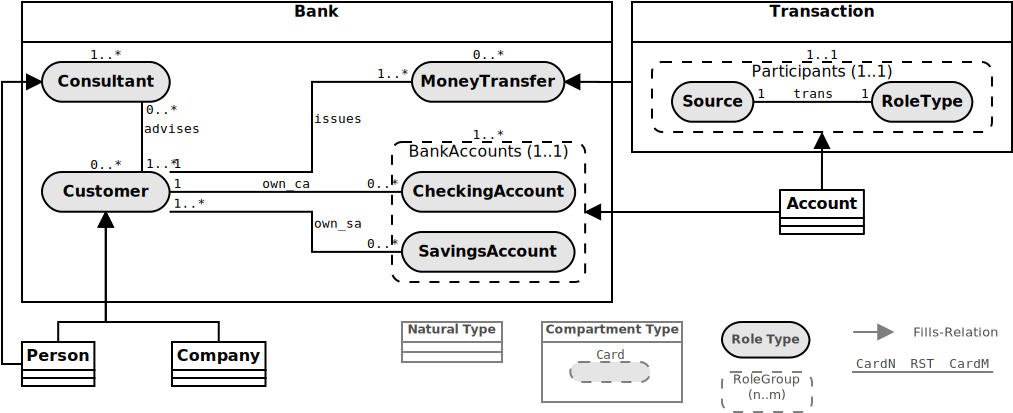
\includegraphics[width=\textwidth]{Bank-full-constraints}
  \caption{Graphical notation of a CROM for an banking application}
  \label{fig:bank}
\end{figure}

In our definitions, we omit to precisely define the graphical notation as they are not relevant for
reasoning on CROMs and refer to~\cite{KBG-SLE15}.

Next, we introduce instances of role-based models. An instance is based on a non-empty domain,
where each element is of exactly one type, i.e.\ a natural type, a \rosirole type or a compartment
type. Objects playing \rosirole in a compartment are collected in a ternary relation \plays and the
relation of two \rosiroles via a relationship type in a compartment is stored in \links.


\begin{definition}[Compartment Role Object Instance, Satisfiability]\label{def:scroi}
  Let $\Sigma = (\NT, \RT,$ $\CT,\RST)$ be a vocabulary.  Then, a
  \emph{Compartment Role Object Instance \I over $\Sigma$ (\SCROI)} is a tuple
  $\I=(\Gamma^{\I},\type,\plays,\links)$, where
  \begin{itemize}
  \item $\Gamma^{\I}$ is a non-empty domain, and
  \item $\type:\Gamma^{\I}\to\NT\cup\RT\cup\CT$ is a total function.
  \end{itemize}
  Based on the \type-function, we can partition the domain into the set \Nsf of \emph{naturals},
  i.e.\ all instances of any natural type, the set \Rsf of \emph{\rosiroles}, i.e.\ all instances of
  any \rosirole type, and the set \Csf of \emph{compartments}, i.e.\ all instances of any
  compartment type. Furthermore, the set \Osf of \emph{objects} denote all domain elements that are
  eligible to play a \rosirole, i.e.\ all naturals and compartments.
  \begin{align*}
    \Nsf & \coloneqq \{d \in \Gamma^{\I} \mid \type(d) \in \NT\} \\
    \Rsf & \coloneqq \{d \in \Gamma^{\I} \mid \type(d) \in \RT\} \\
    \Csf & \coloneqq \{d \in \Gamma^{\I} \mid \type(d) \in \CT\} \\
    \Osf & \coloneqq \Nsf \cup \Csf
  \end{align*}
  %
  Now, \plays and \links are defined as follows:
  \begin{itemize}
  \item $\plays \subseteq \Osf\times\Csf\times\Rsf$ is a ternary relation, and
  \item $\links: (\RST\times\Csf) \to \powerset{\Rsf\times\Rsf}$ is a total function.
  \end{itemize}
  %
  Furthermore, %
  the set $T^{\I}$ of all elements of type $T\in(\NT\cup\RT\cup\CT)$, %
  the set \Osf[\I,c] of all objects playing a role in $c$, %
  the set \Osf[\I,c,\rt] of all objects playing an \rt-role in $c$, and %
  the set \Rsf[\I,c] of all roles played in $c$ %
  are defined as follows:
  \begin{align*}
    T^{\I}     & \coloneqq \{d \in \Gamma \mid \type(d) = T\},\\
    \Osf[\I,c] & \coloneqq \{o \in \Osf \mid \text{there is some $r$ with $(o,c,r) \in \plays$}\}, \text{ and}\\
    \Osf[\I,c,\rt] & \coloneqq \{o \in \Osf \mid \text{there is some $r$ with $(o,c,r) \in \plays$
                     and $r\in\rt^{\I}$}\}\\
    \Rsf[\I,c] & \coloneqq \{r \in \Rsf \mid \text{there is some $o$ with $(o,c,r) \in \plays$}\}.
  \end{align*}
  %
  A \SCROI{} \I \emph{satisfies} a \SCROM{} \Mmc, denoted by $\I\models\Mmc$, if it has the following
  properties:
  \begin{enumerate}
  \item The \plays-relation respects \fills, i.e.~for each tuple $(o,c,r)\in\plays$ the type of $o$
    fills the type of $r$:
    \begin{align*}
      \{(o,r)\mid(o,\cdot,r)\in\plays\}\ \subseteq\ \{(o,r)\mid\text{there exists
        $(T,\rt)\in\fills$ s.t. $o\in T^{\I}$, $r\in \rt^{\I}$}\}.
    \end{align*}
  \item The \plays-relation respects \parts, i.e.~for each tuple $(o,c,r)\in\plays$ the type of $r$
    participates in the type of $c$:
    \begin{align*}
      & \{(c,r)\mid(\cdot,c,r)\in\plays\}\\
      & \quad \subseteq\ \{(c,r)\mid \text{there exists $\ct \in \CT$, $\rt \in \RT$ s.t. $c \in
        \ct^{\I}$, $r \in \rt^{\I}$, $\rt \in \parts(\ct)$}\}.
    \end{align*}
  \item Each object can only play one role of each role type in each compartment:
    \begin{align*}
      \{(o,c,r),(o,c,r')\}\subseteq\plays \textImplies \type(r)\neq\type(r').
    \end{align*}
  \item Each role is played by exactly one object in exactly one compartment:
    \begin{align*}
      |\{(o,c)\mid(o,c,r)\in\plays\}| = 1 \quad\text{for all $r \in \Rsf$}.
    \end{align*}
  \item Roles occurring in the image of \links are played in the associated compartment, i.e.\ for
    each $(r_{1},r_{2})\in\links(\rst,c)$ there exists objects that play $r_{1}$ and $r_{2}$ in $c$:
    \begin{align*}
      \{r_{1} \mid (r_{1},\cdot) \in \links(\cdot,c)\} \cup \{r_{2} \mid (\cdot,r_{2}) \in \links(\cdot,c)\} \ \subseteq\ \{r\mid(\cdot,c,r)\in\plays\}.
    \end{align*}
  \item The \links-function respects \rel, i.e.\ for each $(r_{1}, r_{2}) \in \links(\rst, \cdot)$ the
    types of $r_{1}$ and $r_{2}$ are related via \rst:
    \begin{align*}
      (r_{1},r_{2}) \in \links(\rst, \cdot) \textImplies \rel(\rst)=(\type(r_{1}),\type(r_{2})).
    \end{align*}
  \end{enumerate}

  A \SCROM{} \Mmc is \emph{satisfiable} if there exists any \SCROI{} \I such that $\I\models\Mmc$. 
\end{definition}

We say that $r$ is an $\rt$-role and $c$ is a $\ct$-compartment if, respectively,
$\type(r) = \rt \in \RT$ and $\type(c) = \ct \in \CT$.  Furthermore, \emph{$o$ plays $r$ in $c$} and
$o$ is the \emph{player} of $r$ if $(o,c,r) \in \plays$, and \emph{$r_{1}$ is linked to $r_{2}$ via
  $\rst$ in $c$} if $(r_{1}, r_{2}) \in \links(\rst, c)$.

% Again, it is easy to verify that our definition of a \SCROI satisfying a \SCROM is equivalent to the
% definition of~\cite{KBG-SLE15}.
% Since the \plays-relation respects the \fills- and the \parts-relation, if $o$ plays an \rt-role in
% a \ct-compartment, then the type of $o$ must fill \rt and \rt must participate in \ct. If $o$ plays
% $r_{1}$ and $r_{2}$ in $c$ then $r_{1}$ and $r_{2}$ must have different types, because each object
% can only play one role of each type in the same compartment. Moreover, for each role there exists
% exactly one object that plays it and one compartment where it is played in. In contrast to the
% formalisation in~\cite{KBG-SLE15} we omit $\varepsilon$-roles, but roles that are linked via a
% relationship type are both played in the same compartment and must be instances of the correct types
% since \links respects \rel.  Thus, equations (6) to (11) of~\cite{KBG-SLE15} are satisfied.

Before we investigate how the information about a \SCROM can be encoded in a description logic
ontology, we have to discuss the main reasoning tasks for role-based models. The arguably most
apparent question is, given a \SCROM{} \Mmc and a \SCROI{} \I, whether \I is compliant with
\Mmc. But as this task rather belongs to the area of model checking, we will not focus on that
problem in this thesis.
%
Instead, given a \SCROM{} \Mmc, it ismore interesting whether there exists any \SCROI that is
compliant with \Mmc.  Additionally, we often want to know for a specific \SCROM{} \Mmc whether there
exists a compliant \SCROI that fulfills certain assertions, e.g.\ that a role of a certain type is
played.  To express this assertional knowledge, we introduce a so-called \SCROA, a set of
assertions which should additionally be satisfied by a \SCROI.

\begin{definition}[$\Sigma$-Compartment Role Object Assertions] \label{def:scroa} Let
  $\Sigma = (\NT, \RT, \CT, \RST)$ be a vocabulary and let \INDC and \IND be two non-empty, disjoint
  sets of meta and object individual names disjoint from $\Sigma$.  A \emph{Compartment Role Object
    Assertion over $\Sigma$} is of the form
  \begin{itemize}
  \item $T(c)$ with $T\in\CT$ and $c\in\INDC$ (\emph{meta type assertion}),
  \item $T(a,c)$ with $T \in \NT \cup \CT \cup \RT$, $a\in\IND$ and $c\in\INDC$ (\emph{object type assertion}),
  \item $\playass(a_{1}, c, a_{2})$ with $a_{1}, a_{2} \in \IND$ and $c\in\INDC$ (\emph{plays assertion}), or
  \item $\linkass(\rst, c, a_{1}, a_{2})$ with $\rst \in \RST$ and  $a_{1}, a_{2} \in \IND$ and
    $c\in\INDC$ (\emph{link assertion}). 
  \end{itemize}

  A \emph{set of Compartment Role Object Assertions \A over $\Sigma$ (\SCROA)} is a set of such
  assertions.
  %
  We extend the \SCROI{} \I to additionally map individual names to domain elements, e.g.\
  $a\in\IND$ and $c\in\INDC$ are
  mapped to a domain elements $a^{\I} \in \Gamma^{\I}$ and $c^{\I} \in \Gamma^{\I}$. A \SCROI{} \I \emph{satisfies an assertion
    $\alpha$}, denoted by $\I\models\alpha$, if the following conditions hold:
  \begin{itemize}
  \item if $\alpha = T(c)$, then $c^{\I} \in T^{\I}$,
  \item if $\alpha = T(a, c)$, then $a^{\I} \in T^{\I} \cap (\Osf\cup\Rsf[\I,c])$,
  \item if $\alpha = \playass(a_{1}, c, a_{2}, )$, then
    $(a_{1}^{\I}, c^{\I}, a_{2}^{\I}) \in \plays$, and
  \item if $\alpha = \linkass(\rst, c, a_{1}, a_{2})$, then there exist $r_{1}, r_{2} \in \Rsf$ with
    $(a_{1}, c, r_{1})\in\plays$, $(a_{2}, c, r_{2})\in\plays$ and
    $(r_{1}^{\I}, r_{2}^{\I}) \in \links(\rst, c^{\I})$.
  \end{itemize}

  A \SCROI{} \I \emph{satisfies \A}, denoted by $\I\models\A$ if it satisfies all assertions
  in \A.
\end{definition}

Note here that the link assertion asserts for two objects that they play roles which are related via
\rst, and not that the objects themselves are related.
%
Moreover, without any assertions there always exists a trivial CROI that satisfies \Mmc with the
singleton set $\Gamma = \{o\}$ where the type of $o$ is some natural type, and \plays and \links are
empty sets. Therefore, we introduce in the next section further constraints.


\subsection{Constraint Level}
\label{sec:constraint-level}

When modelling a domain of interest, not only the type of an object defines whether that object is
allowed to play a certain role. In~\cite{KBG-SLE15} additional constraints were introduced. These
can be divided into four groups.

\emph{Role constraints} are the first category of constraints which state, for example, that roles
mutually exclude each other or playing one role implies playing another role. More general these
constraints are formalised with so-called \emph{role groups}. These consist of a set of role types
(or again role groups), a lower and an upper bound. An object fulfills a role group if it plays at
least the lower and at most the upper bound of roles from the set of role types.

\begin{definition}[Syntax of role groups]\label{def:syntax-role-groups}
  Let \RT be a set of role types. The set of \emph{role groups over \RT} is the smallest such that
  \begin{itemize}
  \item if $\rt \in \RT$, then \rt is an (\emph{atomic}) role group, and
  \item if $A_{1}$, \dots, $A_{n}$ are role groups, $k,\ell \in \nat$, then $(\{A_{1}, \dots, A_{n}\},
    k,\ell)$ is a (\emph{complex}) role group.
  \end{itemize}
  \emph{Atoms} of a role group $A$ are defined as:
  \begin{align*}
    \atom(A) & \coloneqq
               \begin{cases}
                 \{\rt\} & \text{if $A = \rt \in \RT$}\\
                 \bigcup_{i=1}^{n} \atom(A_{i}) & \text{if $A = (\{A_{1}, \dots, A_{n}\},k,\ell)$}.
               \end{cases}
  \end{align*}
  Role groups that occur within other role groups are called \emph{nested}.
\end{definition}

The semantics of a role group are based on a \SCROI and are locally evaluated for each domain
element and each compartment.  The interpretation function $\cdot^{\I,c,o}$ calculates recursively
whether an object fulfills the role group.

\begin{definition}[Semantics of role groups]\label{def:semantics-role-groups}
  Given a \SCROI{} \I, the semantics of a role group~$A$ is defined for an object $o \in \Osf$ in
  $c \in \Csf$ as follows:
  \begin{align*}
    A^{\I,c,o} & \coloneqq 
                 \begin{cases}
                   1 & \text{if $A = \rt\in\RT$ and $o$ plays an \rt-role in $c$, or} \\
                     & \text{if $A = (\{B_{1},\dots,B_{n}\},k,\ell)$ and $k \leq \sum_{i=1}^{k}
                     B_{i}^{\I,c,o} \leq \ell$, and}\\
                   0 & \text{otherwise.}
                 \end{cases}
  \end{align*}

  If $A^{\I,c,o} = 1$, we say that $o$ fulfills $A$ in $c$.
\end{definition}

\noindent
Basic role constraints, for example as defined in~\cite{RiGr-OOPLSLA98}, i.e.\ role implication,
role equivalence and role prohibition, can be expressed with role groups as well as much more
complex ones. In fact, any propositional formula can be emulated with role groups.

\begin{proposition}
  Let $\varphi$ be some propositional formula. Then, there exists a role group $A_{\varphi}$ such
  that $\varphi$ is satisfiable if and only if $A_{\varphi}$ can be fulfilled.
\end{proposition}
\begin{proof}
  We define $A_{\varphi}$ inductively as follows:
  
  \vspace{\topsep}
  \begin{tabular}{@{ if }l@{\quad then\quad }l}
    $\varphi = p$ & $A_{\varphi} \coloneqq \rt[p]$,\\
    $\varphi = \lnot \psi$ & $A_{\varphi} \coloneqq (\{A_{\psi}\}, 0, 0)$,\\
    $\varphi = \psi_{1}\land\psi_{2}$ & $A_{\varphi} \coloneqq (\{A_{\psi_{1}}, A_{\psi_{2}}\}, 2, 2)$, and\\
    $\varphi = \psi_{1}\lor\psi_{2}$ & $A_{\varphi} \coloneqq (\{A_{\psi_{1}}, A_{\psi_{2}}\}, 1, 2)$.
  \end{tabular}
  \vspace{\topsep}
  
  \noindent
  Next, we establish a 1-to-1-relation between a valuation $\rho$ for $\varphi$ and a
  $\Sigma$-CROI{} \I. For every propositional variable $P_{i}$ occurring in $\varphi$, we introduce
  a role type \rt[i] and assume that $o$ plays an \rt[i]-role iff $\rho(P_{i}) = \true$. By
  induction, it follows that $\rho(\varphi) = \true$ iff $o$ fulfills $A_{\varphi}$.
\end{proof}


The next category of constraints are \emph{occurrence constraints}. These state how often a role
type or role group must at least or at most be played in a compartment. Therefore, we introduce the
notion of a \emph{cardinality}, a pair $(k,\ell)\in\nat\times\natinf$ with $k\leq\ell$. We usually
denote cardinalities by $(k..\ell)$. Since role types are also atomic role groups, it suffices to
specify occurrence constraints for role groups.
%
Similar to multiplicities specified for associations in UML class diagrams, we specify
\emph{cardinality constraints} for relationship types. They express how often a role of certain type
must be related via a relationship type to some other role type.

Last but not least, the category of \emph{intra-relationship type constraints} imposes constraints on the
players of roles which are related via a relationship type. For example, stating that the
relationship type $\mathsf{isAncestorOf}$ between the role types $\mathsf{Parent}$ and
$\mathsf{Child}$ is transitive assures the existence of a respective link between a grandparent and
a grandchild. Note here, that the transitivity is evaluated over the players and not the roles
themselves.

\begin{definition}[Constraint set]
  Let $\Sigma = (\NT, \RT, \CT, \RST)$ be a vocabulary, let \RG be the set of role groups over \RT
  and let $\Card \coloneqq \nat \times \natinf$ be the set of cardinalities.  Then, a
  \emph{$\Sigma$-Compartment Role Object Constraint Set (\SCROC) \Cmc} is a tuple $\CC$ where
  \begin{itemize}[topsep=5pt]
  \item $\occur : \CT \to \powerset{\Card \times \RG}$,
  \item $\card : \RST \to \Card \times \Card$, and
  \item $\intra : \RST \to \powerset{\Emc}$ with \Emc being a set of functions of the form
    $e : \powerset{A\times B}\to \{\true, \false\}$ for arbitrary sets $A$, $B$.
  \end{itemize}
  are total functions.  The set of all non-nested role groups that appear in \occur is the set of
  \emph{top-level role groups \RG*}.
  %
  A \SCROC{} \Cmc is \emph{compliant} to a \SCROM if all atoms of a role group that is in the occurrence
  constraints of a compartment type participate in that compartment type. 
  %
  Before we define satisfiability, we introduce the following auxiliary functions:
  \begin{align*}
    \Succ(\rst,r,c) & \coloneqq \{r' \in \Rsf \mid (r,r') \in \links(\rst,c)\}, \\
    \Pred(\rst,r,c) & \coloneqq \{r' \in \Rsf \mid (r',r) \in \links(\rst,c)\}\text{, and} \\
    \links^{*}(\rst,c) & \coloneqq \{ (o_{1}, o_{2}) \mid (r_{1}, r_{2}) \in \links(\rst,c) \text{
                         and } (o_{1}, c, r_{1}), (o_{2}, c, r_{2}) \in \plays\}.
  \end{align*}
  %
  A \SCROI{} \I \emph{satisfies \Cmc}, denoted by $\I\models\Cmc$, if it has the following
  properties:
  \begin{enumerate}
  \item All occurrence constraints are respected, i.e.\ if $(k..\ell,A) \in \occur(\ct)$, then in
    every \ct-compartment there must exist at least~$k$ and at most~$\ell$ objects that fulfill role
    group~$A$:
    \begin{align*}
      ((k,\ell),A) \in \occur(\ct) \textImplies  \ct^{\I} \subseteq \left\{c \in \Csf \mmid k \leq \sum\nolimits_{o\in\Osf[\I,c]}
      A^{\I,c,o} \leq \ell \right\}
    \end{align*}
  \item All top-level \rosirole groups must be satisfied, i.e.\ if an object~$o$ plays an \rt-role and
    \rt is an atom of a top-level \rosirole group~A, then $o$ must fulfill~$A$:
    \begin{align*}
      & (o,c,r) \in \plays \text{, } r \in \rt^{\I} \text{ and } \rt \in \atom(A) \textImplies
      A^{\I,c,o} = 1\text{,} \\
      & \hspace{8cm} \text{for all $o \in \Osf$, $A \in \RG*$}.
    \end{align*}
  \item All cardinality constraints are respected, i.e.\ every \rosirole that is played in a
    compartment~$c$ and whose type is either the domain or the range of a relationship type~\rst
    with $\card(\rst) = (i..j, k..\ell)$ must have at least~$k$ and at most~$\ell$ \rst-successors
    in~$c$ or at least~$i$ and at most~$j$ \rst-predecessors in~$c$, respectively:
    \begin{align*}
      & (\cdot,c,r) \in \plays \text{, } r \in \rt[1]^{\I} \text{, } \rel(\rst) = (\rt[1], \cdot) \text{ and
        } \card(\rst)=(\cdot,k..\ell)\\
      & \qquad \textImplies k \leq | \Succ(\rst,r,c) | \leq \ell
    \end{align*}
    \begin{align*}
      & (\cdot,c,r) \in \plays \text{, } r \in \rt[2]^{\I} \text{, } \rel(\rst) = (\cdot, \rt[2]) \text{ and
        } \card(\rst)=(i..j,\cdot)\\
      & \qquad \textImplies i \leq | \Pred(\rst,r,c) | \leq j
    \end{align*}

  \item All intra-relationship type constraints are respected, i.e.\ every function $\fsf \in
    \intra(\rst)$, evaluated over the players of the roles related via \rst, must return \true:
    \begin{align*}
      & \fsf \in \intra(\rst) \textImplies \fsf(\links^{*}(\rst,c)) = \true \\
      & \qquad\text{for all $c$ in $\ct^{\I}$ s.t.\ \rst participates in \ct}.\qedhere
    \end{align*}
  \end{enumerate}
\end{definition}

The definition of satisfying a constraint model in~\cite{KBG-SLE15} is, neglecting
$\varepsilon$-roles, exactly reflected in the above definition. With constraints being formally
introduced, we can complete the CROM for the banking application of Example~\ref{ex:bank-crom} and Figure~\ref{fig:bank}.

\begin{example}
  We first define the complex \rosirole groups that occur in our example. The \rosirole group
  $\mathsf{Participants}$ in the context of an transaction ensures that a single account cannot be
  both the source and the target of an transaction. The \rosirole group $\mathsf{BankAccounts}$
  states the same for savings and checking accounts in the context of a bank. A single account
  cannot attain both \rosiroles simultaneously. 
  \begin{align*}
    \mathsf{Participants} & \coloneqq (\{\mathsf{Source}, \mathsf{Target}\},1,1)\\
    \mathsf{BankAccounts} & \coloneqq (\{\mathsf{SavingsAccount}, \mathsf{CheckingAccount}\},1,1)
  \end{align*}
  We next analyse the occurrence constraints. In our example a bank can only exists if it contains
  at least on consultant and one bank account. A transaction has exactly one source or
  target\footnote{Note here, that this small modelling error is made on purpose. We will discuss its
    logical implications later. Actually a transaction has exactly one source \emph{and} one target,
    and, hence, exactly two participants.}.
  \begin{align*}
    \occur(\mathsf{Bank}) & \coloneqq \{(1..\infty, \mathsf{Consultant}), (1..\infty, \mathsf{BankAccounts})\}\\
    \occur(\mathsf{Transaction}) & \coloneqq \{(1..1,\mathsf{Participants})\}
  \end{align*}
  For the appearing cardinality constraints we assume the following in the context of a bank. A
  consultant must advise at least one customer but not every customer necessarily needs a
  consultant. A customer does not need to have any bank account, but every bank account needs to
  have an owner. A checking account has exactly one owner, a savings account could have several. A
  money transfer is issued by exactly one customer and each customer issues at least one money
  transfer. In the context of a transaction, there is a one-to-one connection between source and
  target. 
  \begin{align*}
    \card(\mathsf{advises}) & \coloneqq (0..\infty,1..\infty)\\
    \card(\mathsf{own\_ca}) & \coloneqq (1..1,0..\infty)\\
    \card(\mathsf{own\_sa}) & \coloneqq (1..\infty,0..\infty)\\
    \card(\mathsf{issues}) & \coloneqq (1..1,1..\infty)\\
    \card(\mathsf{trans}) & \coloneqq (1..1,1..1)
  \end{align*}
  The intra-relationship type constraints are empty since we do not have such constraints in our
  example. 
\end{example}




At last we combine all parts of the role-based system into one \emph{constrained
  $\Sigma$-compartment Object Role Model}.

\begin{definition}[Constrained $\Sigma$-Compartment Role Object Model]
  \label{def:constrained-sigma-crom}
  Let $\Sigma = (\NT, \RT,$ $ \CT, \RST)$ be a vocabulary, let~\Mmc be a \SCROM, let~\Amc be a \SCROA
  and let~\Cmc be a \SCROC.
  %
  Then, a \emph{Constrained $\Sigma$-Compartment Role Object Model \SCCROM} is the tuple
  $\Kmc = (\Mmc, \Amc, \Cmc)$.

  The \emph{satisfiability problem} for \SCCROM{s} is the problem of deciding for a given \SCCROM{}
  $\Kmc = (\Mmc, \Amc, \Cmc)$ whether there exists a \SCROI that satisfies~\Mmc,~\Amc and~\Cmc.
\end{definition}



\section{Requirements for Logical Formalism}
\label{sec:requirements-and-CDLs}

Basically every large software project starts with modelling the application domain in UML. While
UML is the de facto standard as modelling language, it has several drawbacks. First of all, it has
no formally defined semantics~\cite{FrEL-CSI98}. While UML meta-models capture the precise syntax of
concepts used for modelling, they do little for answering questions of how to interpret non-trivial
UML diagrams.  For example, if one wants to map UML class diagrams to a logical formalism to be able
to reason about these diagrams, one takes certain assumptions about the intended meaning of the
occurring elements. Then a domain expert modelling some application has to trust that the logician
constructed the mapping with the same semantics in mind. Nevertheless, over the last years several
approaches for formal frameworks to reason on UML
arose~\cite{Eva-WIFT98,CaCG-ISMIS02,StMS-UML03,SiSJ-OBJ04,BeCG-AI05,SiBH-IJSEKE08,AhNa-ICET10}, from
which we can adapt some ideas, e.g. to model attributes of a~UML class with~DL roles and how
multiplicities of associations are modelled in~\cite{CaCG-ISMIS02}.

Besides that, UML lacks expressive power to model context-dependent domains. There also exist some
work on extending UML in that direction~\cite{ShB-ICMB05}, but here the semantics are even more ambiguous.
Therefore, we focus on role-based models that are based on CROM since it has both a well-defined,
formal semantics and the means to formulate the necessary concepts accordingly.

The only drawback might be the expressive restrictions of ``classical'' description logics as
explained in the introduction. Standard DLs cannot formalise contextual knowledge in a proper way
which is crucial for role-based systems.  In the recent years many different approaches and
extensions of DLs have been proposed~\cite{BoGH-ISWC03, BoGH-WS04, BeAF-ADVIS06, BaVS-ModOnt09, BaKP-JWS12,
  CePe-IJCAR14, CePe-JAR17}.  However, many were tailored to different goals, for example to support
context-specific reuse of ontologies or enable probabilistic reasoning. Additionally, these
approaches have a quite different intuition of what a context exactly is. In most cases it is simply
a finite set of names.  Serafini et al.~\cite{SeHo-JWS12} defines contexts by a set of
attribute-value declarations, one for each \emph{dimension}, e.g.\ time, topic or location to name a
few. There is only one context for each dimensional vector whereas there can exist many instances
of one compartment type.  Furthermore, except a coverage relation, one can hardly express any other
knowledge about the contexts such as the relational structure between them.  Hence, these
approaches seem not appropriate to model CROMs.

A far more promising formalism is the description logic of context \klarALC~\cite{KG-JELIA10, KG16}
mentioned in Section~\ref{sec:adding-cont-concepts}. Klarman et al.\ follow the ideas of McCarthy's
formalization of contexts~\cite{McC-ACM87,McC-IJCAI93} where contexts are formal objects, that have
properties and can be described, and that are organised in a relational structure.  This results in
a very expressive, two-dimensional description logic with strong interactions between the object and
the context level allowing to express information within a context that is valid in some other
context.  While transcending object knowledge through contexts is very important in the general
application of contextualised knowledge, it is complexity-wise very costly, especially in the
presence of rigid roles where the consistency problem becomes undecidable.

By restricting that interaction to a top-down view of contexts, we can retain decidability. From the
meta or context level, we can impose axioms that must hold within a certain context, but on the object
level, i.e.\ within a context, we cannot ``look outside''.
%
When formalizing compartments, this is exactly the needed expressiveness. For each compartment type
we want to specify the constraints which must hold within a compartment of that type.
%
This analysis led to the construction of \LMLO.
In Section~\ref{sec:adding-cont-concepts}, we showed that \ALCALC is indeed a sublogic of \klarALC.
We will now present how a CROM can be represented in \LMLO.


\section{Representing Role-Based Models}
\label{sec:representating-role-based-models}

We would like to emphasise here once again that checking well-formedness of a \SCROM{}~\Mmc and
compliance of a constraint set with \Mmc is not considered here, because these are purely
syntactical checks and no reasoning is necessary. Furthermore, checking whether a given \SCROI
satisfies \Mmc is also not the considered task as it rather belongs to the area of model checking
and is in the scope of this thesis. More interesting is whether there exists such a \SCROI at all.
Then, we can additionally test if certain axioms are entailed or whether specific role types can be
played since these questions can be reduced to the satisfiability problem. Thus, the main objective
is, given a \SCCROM{} \Kmc, to construct an \LMLO-ontology $\Bmf_{\Kmc}$ such that $\Bmf_{\Kmc}$ is
consistent iff \Kmc is satisfiable.

The general idea is to model compartment types as concepts on the meta level, and objects playing a
\rosirole, the relationship types as well as all the constraints within a compartment type on the
object level. For this, we introduce o-concepts for natural types and \rosirole types and a special
object role \plays. The fills relation is transformed into corresponding domain and range axioms for
\plays.

Here, we made a first design decision on how to express that a \rosirole is played within a
compartment. There are two possibilities, depicted in Figure~\ref{fig:two-ways-to-play-roles}, which
we already showed in Example~\ref{ex:nfl-with-contexts}. On the one hand, we can introduce
an o-concept $\mathsf{Coach}\in\RT$ and elements playing a $\mathsf{Coach}$-\rosirole are in the
extension of \rt (such as Mike McCarthy playing the \rosirole of a coach in the left side of
Figure~\ref{fig:two-ways-to-play-roles}). Here, an object $o$ and a \rosirole $r$ with
$(o,\cdot,r)\in\plays$ would be mapped to a single element $d$ in the object interpretation for that
compartment. This variant is close to the ontological nature of \rosiroles where an entity is in the
extension of a \rosirole, seen as unary predicate, if this entity plays that \rosirole. On the other
hand, we can introduce the o-concept $\mathsf{Coach}$ as well but disjoint from $\mathsf{Person}$
and we additionally introduce an object role \plays and elements playing an
$\mathsf{Coach}$-\rosirole have a \plays-successor that is in the extension of $\mathsf{Coach}$
(such as Mike playing the \rosirole of a coach in the left side of
Figure~\ref{fig:two-ways-to-play-roles}).  This is closer to the semantics of \SCROI{s}, but
introduces new object domain elements for each \rosirole that is played.  Still, we chose the latter
variant, since later we need to count the number of \rosiroles to assure occurrence and
cardinality constraints. In~DLs, this can be done via qualified number restrictions.

\begin{figure}
  \centering
  \begin{tikzpicture}
    \node[node,label={[align=left]270:\textit{MikeMcCarthy},\\ $\mathsf{Coach}$}] (mmc) at (-2,0){};
    \node[node,label={[align=left]270:\textit{MikeMcCarthy}}] (ar) at (2,0){};
    \node[node,label={[align=right]south:$\mathsf{Coach}$}] (qb) at (5,0){};
    \draw[edge] (ar) to[bend left=10] node{\plays} (qb);
    \draw[thin] (0,-1.5) to (0,1);
  \end{tikzpicture}
  \caption{Possibilities to formalise objects playing \rosiroles.}
  \label{fig:two-ways-to-play-roles}
\end{figure}

Generally, in a \SCROM, compartments are also allowed to play \rosiroles in other
compartments. Within these other compartments a compartment playing a \rosirole does not behave
differently than a natural. Hence, we have compartment types both as meta concept names, i.e.\ as
contexts in which other objects play \rosiroles, and as object concept types, i.e.\ as objects that
play \rosiroles in a context. In a \SCROM there is a one-to-one relationship, since the compartment
as \rosirole-player and as context is the same object. In our formalism, we cannot establish that
tight connection, but we can assure the existence of contexts of a certain compartment type via a
meta role \nested if objects of that type play \rosiroles. Since we cannot restrict the number of
existing contexts in a nested DL interpretation, this is sufficient for the satisfiability
problem. To distinguish between compartment types as contexts and as objects, we call the former
simply \emph{contexts} and the latter \emph{o-compartments} and introduce a copy \CT* of all
compartment types \CT.

Relationship types are intuitively modelled as object roles. Here, it might be more natural to span these
between the played \rosiroles instead of the players. But due to the one-to-one correspondence
between players and played \rosiroles, we can also construct the relationship types between the
players. In doing so, we can avoid the use of role value maps, which would cause the consistency
problem to become undecidable \cite{Sch89}, to formalise intra relationship type constraints. Even so, we
can only support such constraints that are expressible in the underlying DL.

\Rosirole groups are handled like \rosiroles with an additional axiom stating that ``playing'' a
\rosirole group is equivalent to fulfilling the constraints specified in that \rosirole
group. Furthermore, if an object plays an atom of a top-level \rosirole group, that object must
fulfill the \rosirole group.
%
For the occurrence constraints we introduce a fresh individual name \occurCounter and a object role
\counts and enforce that each played role or fulfilled role group is connected to this
counter. Thereby we can use qualified number restrictions to encode the occurrence constraints.
%
For cardinality constraints, we also utilise number restrictions.

% Ontologically, natural types would be captured as rigid concepts and their attributes, if present, as
% rigid roles, since that information does not change contexts-dependently. In our setting, rigidity
% has no influence on the consistency, and neglecting it decreases the computational complexity
% exponentially in the size of the input. Additionally, the case with rigid names can be handled quite
% similar and we come back to it in Section~\ref{sec:going-beyond-crom}.

To sum up, we consider the object signature $\Osig=(\OC,\OR,\OI)$ and the meta signature
$\Msig=(\MC,\MR,\MI)$ such that
\begin{itemize}
\item $\CT \subseteq \MC$, since every compartment type is a meta concept,
\item $\nested \in \MR$, to assure the existence of compartments that play \rosiroles,
\item $\NT\cup\CT* \subseteq \OCR$, since every natural type and every o-compartment type are rigid
  object concepts,
\item $\RT\subseteq\OCF$, since every \rosirole type is a flexible object concept
\item $\plays\in\ORF$, to express the \plays-relation, 
\item $\RST \subseteq \ORF$, since every relationship type is an object role,
\item $\occurCounter \in \OI$ and $\counts\in\ORF$, to express the occurrence constraints, and
\item $\INDC\in\MI$ and $\IND\in\OI$, to interpret individual names on their respective level. 
\end{itemize}
Additionally, we introduce the following object concept names:
\begin{itemize}
\item $\Ant\in\OCR$ for all objects eligible of playing \rosiroles, i.e.\ naturals and
  o-compartments,
\item $\Art\in\OCF$ for all \rosiroles, and
\item $\Arg\in\OCF$ for all instances of \rosirole groups since we
will consider \rosirole groups of the constraint set similar to \rosiroles.
\end{itemize}



% Additionally, we introduce the rigid object concept $\Ant \in \OCR$ for all objects eligible of
% playing \rosiroles, i.e.\ naturals and o-compartments.  and the flexible object concepts
% $\Art\in\OCF$ for all \rosiroles and $\Arg\in\OCF$ for all instances of \rosirole groups since we
% will consider \rosirole groups of the constraint set similar to \rosiroles.

\subsection{A Mapping for the Vocabulary  \texorpdfstring{\ensureboldmath{\Sigma}}{Sigma}}

In the next sections, we present the mapping from \rosirole-based systems into contextualised
description logics in detail.  At first, we express general knowledge about occurring types which is
independent of the specific \SCROM.


\begin{enumerate}

\item Every context belongs to exactly one compartment type.
\begin{align}
  \top & \sqsubseteq \bigsqcup_{\ct\in\CT} \ct \label{eq:compartments-coverage}\\
  \ct[1] \sqcap \ct[2] & \sqsubseteq \bot 
      \text{\qquad\qquad for all $\ct[1], \ct[2] \in \CT$, $\ct[1]\neq\ct[2]$}\label{eq:compartments-disjoint}
\end{align}

\item In every context, every natural or o-compartment and every \rosirole belongs to exactly one type.
\begin{align}
  \top & \sqsubseteq \oax{ \Ant \equiv \bigsqcup_{\nt\in\NT}\nt \sqcup \bigsqcup_{\ct*\in\CT*}\ct*}\label{eq:naturals-coverage}\\
  \top & \sqsubseteq \oax{ \Art \equiv \bigsqcup\limits_{\rt\in\RT}\rt} \label{eq:roles-coverage}\\
  \top & \sqsubseteq \bigsqcap_{\substack{T_{1},\,T_{2}\in\NT\cup\CT*\cup\RT,\\ T_{1} \neq T_{2}}}
      \oax{T_{1} \sqcap T_{2} \sqsubseteq \bot} \label{eq:roles-disjoint}
\end{align}

\item On the object level, an element can either be a \rosirole, a natural or o-compartment, an
instance of a \rosirole group or the individual \occurCounter.
\begin{align}
  %\top & \sqsubseteq \oax{\top \sqsubseteq \Ant \sqcup \Art \sqcup \Arg \sqcup \{\occurCounter\}}\\
  \begin{split}
  \top & \sqsubseteq \oax{\Ant \sqcap \Art \sqsubseteq \bot} 
      \sqcap \oax{\Ant \sqcap \Arg \sqsubseteq \bot}
      \sqcap \oax{\Art \sqcap \Arg \sqsubseteq \bot} \\
    & \qquad \sqcap \oax{\lnot(\Ant \sqcup \Art \sqcup \Arg)(\occurCounter)}
  \end{split}\label{eq:obj-disjoint}
\end{align}

\item Every natural or o-compartment can play at most one \rt-\rosirole in each context and each
  \rosirole must be played by some object.
  \begin{align}
    \top & \sqsubseteq \bigsqcap_{\rt\in\RT} \oax{\Ant \sqsubseteq \atmost{1}{\plays}{\rt}}\label{eq:roletype-played-max-once} \\
    \top & \sqsubseteq \oax{\Art \sqsubseteq \atleast{1}{\plays^{-}}{\top} 
           \sqcap \atmost{1}{\plays^{-}}{\top}}\label{eq:role-is-played-exactly-once}
  \end{align}

\item We formalise a general domain and range restriction for \plays. Only naturals or
  o-compartments can play something, and only \rosiroles or instances of \rosirole groups can be
  played.
  \begin{align}
    \top & \sqsubseteq \oax{ \exists\plays.\top \sqsubseteq \Ant}\label{eq:plays-domain} \\
    \top & \sqsubseteq \oax{\top \sqsubseteq \forall\plays.(\Art\sqcup\Arg)}\label{eq:plays-range}
  \end{align}

\item Finally, if an o-compartment plays a \rosirole in some context, the o-compartment must also
  exist as context.
  \begin{align}
    \lnot\oax{\ct* \sqcap \exists\plays.\top\sqsubseteq\bot} 
    & \sqsubseteq \exists\nested.\ct
      \text{\hspace{3em} for all $\ct* \in \CT*$}\label{eq:nested-cts}
  \end{align}
\end{enumerate}

% \noindent
% In every context, every natural or o-compartment and every \rosirole belongs to exactly one type.
% \begin{align}
%   \top & \sqsubseteq \oax{ \Ant \equiv \bigsqcup_{\nt\in\NT}\nt \sqcup \bigsqcup_{\ct*\in\CT*}\ct*}\label{eq:naturals-coverage}\\
%   \top & \sqsubseteq \oax{ \Art \equiv \bigsqcup\limits_{\rt\in\RT}\rt} \label{eq:roles-coverage}\\
%   \top & \sqsubseteq \bigsqcap_{\substack{T_{1},\,T_{2}\in\NT\cup\CT*\cup\RT,\\ T_{1} \neq T_{2}}}
%       \oax{T_{1} \sqcap T_{2} \sqsubseteq \bot} \label{eq:roles-disjoint}
% \end{align}

% \noindent
% On object level, an element can either be a \rosirole, a natural or o-compartment, an
% instance of a \rosirole group or the individual \occurCounter.
% \begin{align}
%   %\top & \sqsubseteq \oax{\top \sqsubseteq \Ant \sqcup \Art \sqcup \Arg \sqcup \{\occurCounter\}}\\
%   \begin{split}
%   \top & \sqsubseteq \oax{\Ant \sqcap \Art \sqsubseteq \bot} 
%       \sqcap \oax{\Ant \sqcap \Arg \sqsubseteq \bot}
%       \sqcap \oax{\Art \sqcap \Arg \sqsubseteq \bot} \\
%     & \qquad \sqcap \oax{\lnot(\Ant \sqcup \Art \sqcup \Arg)(\occurCounter)}
%   \end{split}\label{eq:obj-disjoint}
% \end{align}

% \noindent
% Next, every natural or o-compartment can only play one \rt-\rosirole in each context and
% each \rosirole must be played by some object.
% \begin{align}
%   \top & \sqsubseteq \bigsqcap_{\rt\in\RT} \oax{\Ant \sqsubseteq \atmost{1}{\plays}{\rt}}\label{eq:roletype-played-max-once} \\
%   \top & \sqsubseteq \oax{\Art \sqsubseteq \atleast{1}{\plays^{-}}{\top} 
%          \sqcap \atmost{1}{\plays^{-}}{\top}}\label{eq:role-is-played-exactly-once}
% \end{align}

% \noindent
% We formalise a general domain and range restriction for \plays. Only naturals or o-compart\-ments
% can play something, and only \rosiroles or instances of \rosirole groups can be played.
% \begin{align}
%   \top & \sqsubseteq \oax{ \exists\plays.\top \sqsubseteq \Ant}\label{eq:plays-domain} \\
%   \top & \sqsubseteq \oax{\top \sqsubseteq \forall\plays.(\Art\sqcup\Arg)}\label{eq:plays-range}
% \end{align}

% \noindent
% Finally, if an o-compartment plays a \rosirole in some context, the o-compartment must also exist as
% context.
% \begin{align}
%   \lnot\oax{\ct* \sqcap \exists\plays.\top\sqsubseteq\bot} & \sqsubseteq \exists\nested.\ct
%       \text{\hspace{3em} for all $\ct* \in \CT*$}\label{eq:nested-cts}
% \end{align}

\subsection{A Mapping for the \texorpdfstring{\SCROM{} \Mmc}{Sigma-CROM M}}

With the general knowledge about the vocabulary $\Sigma$ being set up, we can look into
the translation of the specifications for a given \SCROM{} \MM.

\begin{enumerate}
\item The \fills-relation specifies which natural or compartment types are allowed to play which \rosirole
types. Hence, elements that play a certain \rosirole type can only be naturals or o-compartments of
types which fill that \rosirole type.
\begin{align}
  \top & \sqsubseteq \bigsqcap_{\rt\in\RT}\oax{\exists\plays.\rt \sqsubseteq 
      \bigg( \bigsqcup\nolimits_{(T,\rt)\in\fills} T \bigg)} \label{eq:fills}
\end{align}
Note here, that Equation~\eqref{eq:fills} is sufficient in the sense that in conjunction with
Equations~\eqref{eq:roles-coverage} and~\eqref{eq:plays-range}, it entails that all \plays-successors
of naturals or o-compartments of a specific type are either instances of a \rosirole type that are
filled by that type or instances of a \rosirole group:
\begin{align*}
  \top & \sqsubseteq \bigsqcap_{T\in\NT\cup\CT*}\oax{T \sqsubseteq \forall\plays.
      \bigg(\Arg \sqcup \bigsqcup\nolimits_{(T,\rt)\in\fills} \rt \bigg)}.
\end{align*}

\item Since in a satisfying \SCROI the \plays-relation respects \parts, only \rt-\rosiroles with
$\rt\in\parts(\ct)$ exist in a \ct-context.
\begin{align}
  \ct & \sqsubseteq \oax{\Art \sqsubseteq \bigsqcup_{\rt\in\parts(\ct)}\rt}
      \text{\hspace{3em} for all $\ct\in\CT$} \label{eq:roles-in-compartment}
\end{align}

\item Analogous to \fills restricting the domain and range of \plays, the \rel-function
restricts them for each relationship type.
\begin{align}
  \begin{split}
    \top & \sqsubseteq \oax{\exists\rst.\top\sqsubseteq\exists\plays.\rt[1]} \sqcap
         \oax{\top\sqsubseteq\forall\rst.(\exists\plays.\rt[2])}\\
       & \hspace{7em}\text{for all $\rst\in\RST$ and $\rel(\rst) = (\rt[1],\rt[2])$}
  \end{split}\label{eq:rst-domain-range}
\end{align}
\end{enumerate}
% The \fills-relation specifies which natural or compartment types are allowed to play which \rosirole
% types. Hence, elements that play a certain \rosirole type can only be naturals or o-compartments of
% types which fill that \rosirole type.
% \begin{align}
%   \top & \sqsubseteq \bigsqcap_{\rt\in\RT}\oax{\exists\plays.\rt \sqsubseteq 
%       \bigg( \bigsqcup\nolimits_{(T,\rt)\in\fills} T \bigg)} \label{eq:fills}
% \end{align}
% Note here, that Equation~\eqref{eq:fills} is sufficient in the sense that in conjunction with
% Equations~\eqref{eq:roles-coverage} and~\eqref{eq:plays-range} it entails that all \plays-successors
% of naturals or o-compartments of a specific type are either instances of a \rosirole type that are
% filled by that type or instances of a \rosirole group.
% \begin{align*}
%   \top & \sqsubseteq \bigsqcap_{T\in\NT\cup\CT*}\oax{T \sqsubseteq \forall\plays.
%       \bigg(\Arg \sqcup \bigsqcup\nolimits_{(T,\rt)\in\fills} \rt \bigg)}.
% \end{align*}

% \noindent Since in a valid \SCROI the \plays-relation respects \parts, only \rt-\rosiroles with
% $\rt\in\parts(\ct)$ exist in a \ct-context.
% \begin{align}
%   \ct & \sqsubseteq \oax{\Art \sqsubseteq \bigsqcup_{\rt\in\parts(\ct)}\rt}
%       \text{\hspace{3em} for all $\ct\in\CT$} \label{eq:roles-in-compartment}
% \end{align}

% \noindent Analogous to \fills restricting the domain and range of \plays, the \rel-function
% restricts them for each relationship type.
% \begin{align}
%   \begin{split}
%     \top & \sqsubseteq \oax{\exists\rst.\top\sqsubseteq\exists\plays.\rt[1]} \sqcap
%          \oax{\top\sqsubseteq\forall\rst.(\exists\plays.\rt[2])}\\
%        & \hspace{7em}\text{for all $\rst\in\RST$ and $\rel(\rst) = (\rt[1],\rt[2])$}
%   \end{split}\label{eq:rst-domain-range}
% \end{align}

\noindent Note here, that due to equations~\eqref{eq:compartments-coverage},
\eqref{eq:roles-coverage},~\eqref{eq:roles-disjoint} and~\eqref{eq:roles-in-compartment} and the
fact that \parts' codomain is a partition of \RT, in any context that is not in \ct there are no
\rosiroles of a type the participates in \ct , e.g. the following axiom is entailed for all
$\ct\in\CT$:
\begin{align*}
  \lnot\ct & \sqsubseteq \oax{\bigsqcup_{\rt\in\parts(\ct)}\rt\sqsubseteq\bot}
\end{align*}

\subsection{A Mapping for the \texorpdfstring{\SCROA{} \A}{Sigma-CROA A}}

Next, let \A be a \SCROA. We can translate the different Compartment Role Object Assertions into
meta assertions in \LMLO.

\begin{enumerate}
\item For any meta type assertion of the form $\ct(c)\in\A$ with $\ct\in\CT$ and $c\in\INDC$ the individual $a$ must be a context of
type \ct.
\begin{gather}
  \ct(c)\label{eq:meta-type-assertion}
\end{gather}

\item For any object type assertion $T(a,c)\in\A$ with $T\in\NT\cup\CT\cup\RT$, $a\in\IND$ and $c\in\INDC$ the individual
$a$ is a natural, an o-compartment or \rosirole
  that belongs to the concept $T$ in context $c$.
\begin{gather}
  \oax{T(a)}(c)\label{eq:obj-type-assertion}
\end{gather}

\item A \plays assertion $\playass(a_{1}, c, a_{2}) \in \A$ states that $a_{1}$ plays $a_{2}$
  in $c$.
\begin{gather}
  \oax{\plays(a_{1},a_{2})}(c)\label{eq:plays-assertion}
\end{gather}

\item A \links assertion $\linkass(\rst, c, a_{1}, a_{2}) \in \A$ states that $a_{1}$ and $a_{2}$ play
\rosiroles which are related in $c$ via \rst. Due to the way we modelled relationship types, this is
simply the following axiom: 
\begin{gather}
  \oax{\rst(a_{1}, a_{2})}(c)\label{eq:links-assertion} 
\end{gather}
\end{enumerate}

% For any meta type assertion of the form $\ct(c)\in\A$ with $\ct\in\CT$ and $c\in\INDC$ the individual $a$ must be a context of
% type \ct.
% \begin{gather}
%   \ct(c)\label{eq:meta-type-assertion}
% \end{gather}

% \noindent
% For any object type assertion $T(a,c)\in\A$ with $T\in\NT\cup\CT\cup\RT$, $a\in\IND$ and $c\in\INDC$ the individual
% $a$ is a natural, an o-compartment or \rosirole
%   that belongs to the concept $T$ in context $c$.
% \begin{gather}
%   \oax{T(a)}(c)\label{eq:obj-type-assertion}
% \end{gather}

% \noindent
% A \plays assertion $\playass(a_{1}, c, a_{2}) \in \A$ states that $a_{1}$ plays $a_{2}$
%   in $c$.
% \begin{gather}
%   \oax{\plays(a_{1},a_{2})}(c)\label{eq:plays-assertion}
% \end{gather}

% \noindent
% A \links assertion $\linkass(\rst, c, a_{1}, a_{2}) \in \A$ states that $a_{1}$ and $a_{2}$ play
% \rosiroles which are related in $c$ via \rst. Due to the way we modelled relationship types, this is
% simply the following axiom: 
% \begin{gather}
%   \oax{\rst(a_{1}, a_{2})}(c)\label{eq:links-assertion} 
% \end{gather}
% % This is slightly more complicated as we mapped the
% %   relationship types between the players:
% % \begin{gather}
% %   (\oax{\rst(o_{1}, o_{2})}\sqcap\oax{\plays(o_{1}, a_{1})}\sqcap\oax{\plays(o_{2},
% %     a_{2})})(c)\label{eq:links-assertion} 
% % \end{gather}
% %where w.l.o.g.\ $o_{1}, o_{2}\in\OI\setminus\IND$ are fresh individual names.

\subsection{A Mapping for the \texorpdfstring{\SCROC{} \Cmc}{Sigma-CROC C}}
\label{sec:mapping-constraints}


Let \Cmc be a \SCROC, let $\RG(\Cmc)$ denote the set of all complex \rosirole groups occurring in
\Cmc and let $\RG*(\Cmc) \subseteq \RG(\Cmc)$ denote the set of all complex top-level \rosirole
groups. 

\begin{enumerate}

\item Analogous to \rosiroles, \rosirole groups are disjoint, every instance of a \rosirole group
must be played by some object and every object can either fulfill or not fulfill a \rosirole group.
\begin{align}
  \top & \sqsubseteq \oax{ \Arg \equiv \bigsqcup_{\rg\in\RG(\Cmc)}\rg} 
      \sqcap \bigsqcap_{\substack{\rg[1],\,\rg[2]\in\RG(\Cmc),\\ \rg[1]\neq\rg[2]}} 
      \oax{\rg[1] \sqcap \rg[2] \sqsubseteq \bot}
      \label{eq:rolegroups-coverage-and-disjoint}\\
  \top & \sqsubseteq \oax{\Arg \sqsubseteq \atleast{1}{\plays^{-}}{\top} 
      \sqcap \atmost{1}{\plays^{-}}{\top}}\label{eq:rgs-exactly-one-inverse-plays} \\
  \top & \sqsubseteq \bigsqcap_{\rg\in\RG(\Cmc)} \oax{\Ant \sqsubseteq \atmost{1}{\plays}{\rg}}\label{eq:obj-plays-max-one-rg}
\end{align}

\item Complex \rosirole groups are treated like abstract \rosiroles. An object can ``play'' an instance of
a \rosirole group. This is equivalent to fulfilling that role group. So, the object must ``play''
the required number of containing \rosirole groups.
%
Furthermore, if an object plays a \rosirole whose type is an atom of a top-level \rosirole group,
the object must also fulfill that \rosirole group.
\begin{align}
  \top & \sqsubseteq \bigsqcap_{\substack{\rg\in\RG(\Cmc),\\\rg = (\{A_{1}, \dots, A_{n}\},k,\ell)}}
      \oaxl{\exists\plays.\rg \equiv }
  \begin{aligned}[t]
    & (\atleast{k}{\plays}{(A_{1} \sqcup \dots \sqcup A_{n})}) \\
    &  \quad \sqcap \oaxr{(\atmost{\ell}{\plays}{(A_{1} \sqcup \dots \sqcup A_{n})})}
  \end{aligned}\label{eq:rg-declaration}\\
  \top & \sqsubseteq \bigsqcap_{\rg\in\RG*(\Cmc)}
      \oax{\exists\plays.\bigg(\bigsqcup\nolimits_{\rt\in\atom(\rg)}\rt\bigg)\sqsubseteq \exists\plays.\rg}\label{eq:rg-must-play}
\end{align}

\item Since for the occurrence constraints we only consider objects that play any \rosirole in this
compartment, we assure that fulfilling a \rosirole group implies playing some \rosirole.
\begin{align}
  \top & \sqsubseteq \oax{\exists\plays.\Arg\sqsubseteq\exists\plays.\Art}\label{eq:rgplayer-plays-role}
\end{align}

\item To capture the occurrence constraints we use an object individual name \occurCounter and introduce
an \counts-role from that individual to all \rosiroles and \rosirole group instances. Thus, the
occurrence constraints can be enforced with the help of qualified number restrictions.
\begin{align}
  \top & \sqsubseteq \oax{\Art \sqcup \Arg \sqsubseteq \atleast{1}{\counts^{-}}{\{\occurCounter\}} 
      \sqcap \atmost{1}{\counts^{-}}{\{\occurCounter\}}}\label{eq:counts-decl}\\
  \begin{split}
    \ct & \sqsubseteq \oax{(\atleast{k}{\counts}{\rg})(\occurCounter)}
    \sqcap \oax{(\atmost{\ell}{\counts}{\rg})(\occurCounter)}\\
    & \text{\rlap{\hspace{5em} for all $(k..\ell,\rg)\in\occur(\ct)$, for all $\ct\in\CT$}}
  \end{split}\label{eq:occurrence-constraints}
\end{align}

\item Cardinality constraints restrict the number of \rosiroles that are related to \rosirole via a
relationship type. \Rosiroles whose type is the domain or range of a relationship type \rst for
which there exists a cardinality constraint must have the correct amount of \rst successors or
predecessors, respectively.

\begin{align}
  \top & \sqsubseteq \bigsqcap_{\substack{\rst\in\RST, \\ \rel(\rst) = (\rt[1], \rt[2]), \\
  \card(\rst) = (i..j, k..\ell)}}
  \begin{aligned}[t]
    & \oax{\exists\plays.\rt[1] \sqsubseteq \atleast{k}{\rst}{\top} \sqcap \atmost{\ell}{\rst}{\top}} \\
    & \qquad\qquad \sqcap \oax{\exists\plays.\rt[2] \sqsubseteq \atleast{i}{\rst^{-}}{\top} \sqcap \atmost{j}{\rst^{-}}{\top}}
  \end{aligned}
   \label{eq:last-equation}
\end{align}

\item As mentioned above, because we spanned the relationship types between the players and not between the
\rosiroles, we can model at least some of the intra-relationship type constraints, exactly those
that are expressible in the object logic. In \SHOIQ, these would be transitivity and symmetry. Thus,
we add the following role axioms to the object RBox \RO:
\begin{gather}
  \trans{\rst}  \text{\qquad for all $\transsf\in\intra(\rst)$}\label{eq:rbox-1}\\
  \rst \sqsubseteq \rst^{-} \text{\qquad for all $\symm\in\intra(\rst)$}\label{eq:rbox-2}
\end{gather}
where $\transsf$ and $\symm$ are functions that return $\true$ if and only if the binary relation,
respectively, is transitive or symmetric.  But it is important to note, due to the restriction that
only simple roles are allowed to appear in number restrictions, we cannot impose any cardinality
constraints on the relationship type \rst if \rst is supposed to be transitive.

\end{enumerate}
% Analogous to \rosiroles, \rosirole groups are disjoint, every instance of a \rosirole group
% must be played by some object and every object can either fulfill or not fulfill a \rosirole group.
% \begin{align}
%   \top & \sqsubseteq \oax{ \Arg \equiv \bigsqcup_{\rg\in\RG(\Cmc)}\rg} 
%       \sqcap \bigsqcap_{\substack{\rg[1],\,\rg[2]\in\RG(\Cmc),\\ \rg[1]\neq\rg[2]}} 
%       \oax{\rg[1] \sqcap \rg[2] \sqsubseteq \bot}
%       \label{eq:rolegroups-coverage-and-disjoint}\\
%   \top & \sqsubseteq \oax{\Arg \sqsubseteq \atleast{1}{\plays^{-}}{\top} 
%       \sqcap \atmost{1}{\plays^{-}}{\top}}\label{eq:rgs-exactly-one-inverse-plays} \\
%   \top & \sqsubseteq \bigsqcap_{\rg\in\RG(\Cmc)} \oax{\Ant \sqsubseteq \atmost{1}{\plays}{\rg}}\label{eq:obj-plays-max-one-rg}
% \end{align}

% \noindent
% Complex \rosirole groups are treated like abstract \rosiroles. An object can ``play'' an instance of
% a \rosirole group. This is equivalent to fulfilling that role group. So, the object must ``play''
% the required number of containing \rosirole groups.
% %
% Furthermore, if an object plays a \rosirole whose type is an atom of a top-level \rosirole group,
% the object must also fulfill that \rosirole group.
% \begin{align}
%   \top & \sqsubseteq \bigsqcap_{\substack{\rg\in\RG(\Cmc),\\\rg = (\{A_{1}, \dots, A_{n}\},k,\ell)}}
%       \oax{\exists\plays.\rg \equiv (\atleast{k}{\plays}{(A_{1} \sqcup \dots \sqcup A_{n})}) 
%       \sqcap (\atmost{\ell}{\plays}{(A_{1} \sqcup \dots \sqcup A_{n})})}\label{eq:rg-declaration}\\
%   \top & \sqsubseteq \bigsqcap_{\rg\in\RG*(\Cmc)}
%       \oax{\exists\plays.\bigg(\bigsqcup\nolimits_{\rt\in\atom(\rg)}\rt\bigg)\sqsubseteq \exists\plays.\rg}\label{eq:rg-must-play}
% \end{align}

% \noindent 
% Since for the occurrence constraints we only consider objects that play any \rosirole in this
% compartment, we assure that fulfilling a \rosirole group implies playing some \rosirole.
% \begin{align}
%   \top & \sqsubseteq \oax{\exists\plays.\Arg\sqsubseteq\exists\plays.\Art}\label{eq:rgplayer-plays-role}
% \end{align}

% \noindent
% To capture the occurrence constraints we use an object individual name \occurCounter and introduce
% an \counts-role from that individual to all \rosiroles and \rosirole group instances. Thus, the
% occurrence constraints can be enforced with the help of qualified number restrictions.
% \begin{align}
%   \top & \sqsubseteq \oax{\Art \sqcup \Arg \sqsubseteq \atleast{1}{\counts^{-}}{\{\occurCounter\}} 
%       \sqcap \atmost{1}{\counts^{-}}{\{\occurCounter\}}}\label{eq:counts-decl}\\
%   \begin{split}
%     \ct & \sqsubseteq \oax{(\atleast{k}{\counts}{\rg})(\occurCounter)}
%     \sqcap \oax{(\atmost{\ell}{\counts}{\rg})(\occurCounter)}\\
%     & \text{\rlap{\hspace{5em} for all $(k..\ell,\rg)\in\occur(\ct)$, for all $\ct\in\CT$}}
%   \end{split}\label{eq:occurrence-constraints}
% \end{align}

% \noindent Cardinality constraints restrict the number of \rosiroles that are related to \rosirole via a
% relationship type. \Rosiroles whose type is the domain or range of a relationship type \rst for
% which there exists a cardinality constraint must have the correct amount of \rst successors or
% predecessors, respectively.

% \begin{align}
%   \top & \sqsubseteq \bigsqcap_{\substack{\rst\in\RST, \\ \rel(\rst) = (\rt[1], \rt[2]), \\
%   \card(\rst) = (i..j, k..\ell)}}
%   \begin{aligned}[t]
%     & \oax{\exists\plays.\rt[1] \sqsubseteq \atleast{k}{\rst}{\top} \sqcap \atmost{\ell}{\rst}{\top}} \\
%     & \qquad\qquad \sqcap \oax{\exists\plays.\rt[2] \sqsubseteq \atleast{i}{\rst^{-}}{\top} \sqcap \atmost{j}{\rst^{-}}{\top}}
%   \end{aligned}
%    \label{eq:last-equation}
% \end{align}

% \noindent
% As mentioned above, because we spanned the relationship types between the players and not between the
% \rosiroles, we can model at least some of the intra-relationship type constraints, exactly those
% that are expressible in the object logic. In \SHOIQ, these would be transitivity and symmetry. Thus,
% we add the following role axioms to the object RBox \RO:
% \begin{gather}
%   \trans{\rst}  \text{\qquad for all $\transsf\in\intra(\rst)$}\label{eq:rbox-1}\\
%   \rst \sqsubseteq \rst^{-} \text{\qquad for all $\symm\in\intra(\rst)$}\label{eq:rbox-2}
% \end{gather}
% where $\transsf$ and $\symm$ are functions that return $\true$ if and only if the binary relation,
% respectively, is transitive or symmetric.  But it is important to note, due to the restriction that
% only simple roles are allowed to appear in number restrictions, we cannot impose any cardinality
% constraints on the relationship type \rst if \rst is supposed to be transitive.


Before we establish the desired relation between the CROM and the ontology, we do a short
analysis of the required expressiveness of the meta and the object logic. To state the disjoint union
axioms we need at least~\ALC. As we do not need anything more on the meta level, we can
fix~\LM to be~\ALC. On the object level, we need qualified number restrictions and inverse roles to
assure that every \rosirole is played exactly once. 
%Hence, the minimal object DL is \ALCIQ. 
If we have a single occurrence constraint, we have to add nominals. Transitivity axioms or role
hierarchies are only required if some intra-relationship type constraint specifies a transitive or
symmetric relationship type, respectively. Table~\ref{tab:required-dls} shows a summary of the required DLs.

\begin{table}
  \caption{Summary of required DLs for \LM and \LO}
  \label{tab:required-dls}  \centering
  \begin{tabularx}{0.8\linewidth}{lXl}
    \toprule
    \LO & minimal                                  & \ALCIQ\\
        & with occurrence constraints              & \ALCOIQ\\
        & with intra-relationship type constraints & \SHOIQ\\
    \midrule
    \LM & & \ALC\\
    \bottomrule
  \end{tabularx}
\end{table}

Given a \SCCROM{} \Kmc, we obtain the \ALCSHOIQ ontology
$\Bmf_{\Kmc} = (\Bmc_{\Kmc}, \emptyset,\RO)$ where~$\Bmc_{\Kmc}$ is the conjunction of all meta
axioms from~\eqref{eq:compartments-coverage} to~\eqref{eq:last-equation} and~\RO is the set of all
role axioms~\eqref{eq:rbox-1} and~\eqref{eq:rbox-2}.

\begin{theorem}
  Let $\Kmc = (\Mmc, \Amc, \Cmc)$ be a \SCCROM. Then, \Kmc is satisfiable iff $\Bmf_{\Kmc}$ is consistent.
\end{theorem}
\begin{proof}
  Assume that \Kmc is satisfiable and let \IK denote a \SCROI that satisfies \Mmc, \Amc and
  \Cmc.  We define the set
  $\Delta_{\RT,c}$ of all \rosiroles played in $c$,
  the set $\Delta_{\RG,c}$ of all \rosirole group instances fulfilled in $c$,  and the nested interpretation \JJ as follows:
  \begin{align*}
    \Delta_{\RT,c} & \coloneqq \{r\in\Rsf[\IK] \mid (\cdot,c,r) \in\plays\} \text{\qquad for all $c\in\Csf[\IK]$}\\
    \Delta_{\RG,c} & \coloneqq \{(x,c,y) \in \RG\times\Csf[\IK]\times\Osf[\IK] \mid x^{\IK,c,y}=1\} \text{\qquad for all $c\in\Csf[\IK]$}\\[1ex]
    \Cbb & \coloneqq \Csf[\IK] \\
    \ct^{\J} & \coloneqq \ct^{\IK} \text{\qquad for all $\ct\in\CT$} \\
    \nested^{\J} & \coloneqq \{(c,o) \mid o,c\in\Csf[\IK], (o,c,\cdot)\in\plays\} \\[1ex]
    \Delta^{\J} & \coloneqq \Nsf[\IK] \cup \Csf[\IK] \cup \Rsf[\IK] \cup \bigcup_{c\in\Csf[\IK]}\Delta_{\RG,c} \cup \{d_{\occurCounter}\}\\
    \nt^{\I_{c}} & \coloneqq \nt^{\IK} \text{\qquad for all $\nt\in\NT$} \\
    \ct*^{\I_{c}} & \coloneqq \ct^{\IK} \text{\qquad for all $\ct\in\CT$} \\
    \rt^{\I_{c}} & \coloneqq \rt^{\IK} \cap \Delta_{\RT,c} \text{\qquad for all $\rt\in\RT$} \\
    \rg^{\I_{c}} & \coloneqq \{(\rg,c,y) \mid \rg^{\IK,c,y}=1\} \text{\qquad for all $\rg\in\RG(\Cmc)$}\\
    \Art^{\I_{c}} & \coloneqq \Delta_{\RT,c}\\
    \Ant^{\I_{c}} & \coloneqq \Osf[\IK]\\
    \Arg^{\I_{c}} & \coloneqq \Delta_{\RG,c}\\
    \rst^{\I_{c}} & \coloneqq \{(o_{1},o_{2})\mid\text{ there are $r_{1}$, $r_{2}$ s.t.\
                    $(o_{1},c,r_{1}),(o_{2},c,r_{2})\in\plays$ and}\\
                   & \hspace{3cm}\text{$(r_{1},r_{2})\in\links(\rst,c)$}\}\\
    \plays^{\I_{c}} & \coloneqq \{(o,r) \mid (o,c,r)\in\plays\}\\
                   &\hspace{3cm} \cup \{(o,r{\kern-0.1em}g) \mid r{\kern-0.1em}g =
                     (x,c,o)\in\Delta_{\RG,c}\text{ with $x^{\IK,c,o}=1$}\}\\
    \counts^{\I_{c}} & \coloneqq \{(d_{\occurCounter},y) \mid y\in\Delta_{\RT,c}\cup\Delta_{\RG,c}\}\\
    \occurCounter^{\I_{c}} & \coloneqq d_{\occurCounter}\\
    c^{\J} & \coloneqq c^{\IK} \text{\qquad for $c\in\INDC$}\\
    a^{\I_{c}} & \coloneqq a^{\IK} \text{\qquad for $a\in\IND$}
  \end{align*}
  It is straight forward to show that \J is a model of $\Bmf_{\Kmc}$. Note, that \J respects the
  rigid names since all \nt, \ct*, \Ant and individual names are interpreted the same in every
  world~$c$.
  %
  Axioms~\eqref{eq:compartments-coverage},
  \eqref{eq:compartments-disjoint},
  \eqref{eq:naturals-coverage},
  \eqref{eq:roles-disjoint},
  \eqref{eq:obj-disjoint},
  \eqref{eq:plays-domain},
  \eqref{eq:plays-range},
  \eqref{eq:meta-type-assertion} to~\eqref{eq:obj-plays-max-one-rg},
  \eqref{eq:counts-decl}
  %
  are modelled by construction of \J. Since
  $\Delta_{\RT,c}\subseteq\bigcup_{\rt\in\RT}\rt^{\IK} = \Rsf[\IK]$, \J models \eqref{eq:roles-coverage}.
  %
  Axioms~\eqref{eq:roletype-played-max-once} and~\eqref{eq:role-is-played-exactly-once} are modelled due
  to 3. and 4. of Definition~\ref{def:scroi}. 
  %
  Assume that $c_{1}\in(\lnot\oax{\ct* \sqcap \exists\plays.\top\sqsubseteq\bot})^{\J}$. Hence,
  $\I_{c_{1}}\not\models\ct* \sqcap \exists\plays.\top\sqsubseteq\bot$. Thus, there exists
  $c_{2}\in(\ct* \sqcap \exists\plays.\top)^{\I_{c_{1}}}$. Therefore,
  $(c_{2},c_{1},\cdot)\in\plays$, $(c_{1},c_{2})\in\nested^{\J}$ and $c_{2}\in\ct^{\J}$. Overall, \J
  models Axiom~\eqref{eq:nested-cts}.
  %
  Since \plays respects \fills and \parts, and \links respects \rel, \eqref{eq:fills},
  \eqref{eq:roles-in-compartment} and \eqref{eq:rst-domain-range} are satisfied.
  %
  Axioms~\eqref{eq:rg-declaration} to~\eqref{eq:rgplayer-plays-role} are satisfied due to the
  semantics of \rosirole groups and the fact that all top-level \rosirole groups are satisfied.
  %
  \IK respecting occurrence and cardinality constraints ensures that \J
  models~\eqref{eq:occurrence-constraints} and~\eqref{eq:last-equation}. 
  %
  Finally, the respective intra-relationship constraints imply the satisfaction of \RO.
  
  Conversely, let \JJ denote a model of $\Bmc_{\Kmc}$. W.l.o.g. we can assume that all
  o-compartments that exist also play some \rosiroles. Otherwise we could simply delete them, and
  still have a model. 
  %
  Let $\Delta_{\NT}\subseteq\Delta^{\J}$ and $\Delta_{\CT}\subseteq\Delta^{\J}$ denote,
  respectively, the set of all naturals and the set of all o-compartments, i.e.
  \begin{align*}
    \Delta_{\NT} & \coloneqq \bigcup_{\nt\in\NT} \nt^{\I_{\hat{c}}} \text{, and}\\
    \Delta_{\CT} & \coloneqq \bigcup_{\ct*\in\CT*} \ct*^{\I_{\hat{c}}}
  \end{align*}
  for some $\hat{c}\in\Cbb$.
  %
  Due to \eqref{eq:nested-cts}, there exists a mapping $\mu: \Delta_{\NT}\cup\Delta_{\CT} \to \Delta_{\NT}\cup\Cbb$ which maps
  o-compartments to contexts of respective type, i.e.
  \begin{align*}
    \mu(o) \coloneqq
    \begin{cases}
      o & \text{if $o\in\Delta_{\NT}$, and} \\
      c \text{ such that $c\in\ct^{\J}$} & \text{if $o\in\ct*^{\I_{\hat{c}}}$}.
    \end{cases}
  \end{align*}
W.l.o.g, we can assume that there exist
  sufficiently many contexts $c\in\Cbb$ to assure that $\mu$ preserves the occurrence and
  cardinality constraints, since we could introduce copies of $c$ if necessary.  We define the
  \SCROI{} \I as follows:
  \begin{align*}
    \Gamma^{\I} & \coloneqq \Cbb^{\J} \cup \Delta_{\NT} \cup \bigcup_{c\in\Cbb} \Art^{\I_{c}}\\
    \type(d) & \coloneqq  
               \begin{cases}
                 T & \text{if $T\in\CT$ and $d\in T^{\J}$}\\
                 T & \text{if $T\in\NT\cup\RT$ and $d\in T^{\I_{c}}$ for some $c$}
               \end{cases}\\
    (\mu(o),c,r) \in \plays & \text{\quad iff \quad $(o,r)\in\plays^{\I_{c}}$}\\
    (r_{1}, r_{2}) \in \links(\rst,c) & \text{\quad iff \quad $(o_{1},r_{1}), (o_{2},r_{2}) \in
                                        \plays^{\I_{c}}$ and $(o_{1}, o_{2})\in\rst^{\I_{c}}$}
  \end{align*}
  \I is well-defined and analogous to above one can go through the axioms step by step and show that
  \I satisfies \Kmc, e.g.\ Axiom~\eqref{eq:roles-in-compartment} ensures that \plays respects \parts
  in \I.
\end{proof}

Let us consider once again Example~\ref{ex:bank-crom} and Figure~\ref{fig:bank} to analyse some
implications which can be drawn due to the mapping into description logics.

\begin{example}
  Instead of writing down all axioms of the respective ontology $\Omc_{\Bank}$, we will rather point
  out some interesting inferences. At first we have a look at the \Bank compartment type, the
  \rosirole group \BankAccounts, the relationship types \ownca and \ownsa and the \rosirole type
  \Customer.

  Omitting general axioms, e.g.\ stating that every role or rolegroup instance is played and
  connected to \occurCounter, the following axioms are contained in the ontology, among others:
  \begin{align}
    % \top & \sqsubseteq \oax{\BankAccounts\sqsubseteq\exact{1}{\plays^{-}}{\top}}\\
    \Bank & \sqsubseteq \oax{(\atleast{1}{\counts}{\BankAccounts})(\occurCounter)}\label{eq:counter-bankaccount}\\
    \begin{split}
      \top & \sqsubseteq \oaxl{\exists\plays.\BankAccounts \equiv \atleast{1}{\plays}{(\CheckingAccount\sqcup\SavingsAccount)}}\\
      & \qquad\qquad \sqcap \oaxr{\atmost{1}{\plays}{(\CheckingAccount\sqcup\SavingsAccount)}}
    \end{split}\label{eq:decl-rg-bankaccounts}\\
    \top & \sqsubseteq \oax{\SavingsAccount\sqsubseteq\atleast{1}{\ownsa^{-}}{\top}}\label{eq:card-ownsa}\\
    \top & \sqsubseteq \oax{\CheckingAccount\sqsubseteq\atleast{1}{\ownca^{-}}{\top}}\label{eq:card-ownca}\\
    \top & \sqsubseteq \oax{\exists\ownsa.\top\sqsubseteq\Customer}\label{eq:domain-ownsa}\\
    \top & \sqsubseteq \oax{\exists\ownca.\top\sqsubseteq\Customer}\label{eq:domain-ownca}
  \end{align}
  In any interpretation \J that satisfies $\Omc_{\Bank}$ with $c\in\Bank^{\J}$,
  equations~\eqref{eq:counter-bankaccount} and~\eqref{eq:decl-rg-bankaccounts} entail the existence
  of an element in $\CheckingAccount^{\I_{c}}$ or $\SavingsAccount^{\I_{c}}$. Due to
  \eqref{eq:card-ownsa} and \eqref{eq:card-ownca}, there must be some element ``owning a CA or SA'',
  which must be in $\Customer^{\I_{c}}$ (\eqref{eq:domain-ownsa}
  and~\eqref{eq:domain-ownca}). Hence, the following axiom can be entailed:
\begin{align}
  \Bank & \sqsubseteq \oax{(\atleast{1}{\counts}{\Customer})(\occurCounter)},\label{eq:counter-customer}
\end{align}
stating that the occurrence constraint for \Customer is essentially $1..*$. For the
\Transaction compartment type we have:
\begin{align}
  \Transaction & \sqsubseteq \oax{(\atleast{1}{\counts}{\Participants} \sqcap
                 \atmost{1}{\counts}{\Participants})(\occurCounter)}\label{eq:counter-participants}\\
  \begin{split}
    \top & \sqsubseteq\oaxl{\exists\plays.\Participants \equiv
      \atleast{1}{\plays}{(\Source\sqcup\Target)}}\\
    & \qquad\qquad \sqcap \oaxr{\atmost{1}{\plays}{(\Source\sqcup\Target)}}
  \end{split}\label{eq:decl-rg-participants}\\
  \begin{split}
    \top & \sqsubseteq \oax{\Source \sqsubseteq \atleast{1}{\transBank}{\top} \sqcap
      \atmost{1}{\transBank}{\top}}\\
    & \qquad\qquad \sqcap \oax{\Target \sqsubseteq \atleast{1}{\transBank^{-}}{\top} \sqcap
      \atmost{1}{\transBank^{-}}{\top}} 
  \end{split}\label{eq:card-trans}\\
   \top & \sqsubseteq \oax{\exists\transBank.\top\sqsubseteq\Source} \sqcap \oax{\exists\transBank^{-}.\top\sqsubseteq\Target}\label{eq:domain-range-trans}
\end{align}
Assume that there would be some $d\in\Transaction^{\J}$.  By~\eqref{eq:counter-participants}
and~\eqref{eq:decl-rg-participants}, we know that there exists exactly one element in
$\Source^{\I_{d}}$ or $\Target^{\I_{d}}$. But due to~\eqref{eq:card-trans}
and~\eqref{eq:domain-range-trans}, there must also be an element in $\Target^{\I_{d}}$ or
$\Source^{\I_{d}}$, respectively. This results in two elements in $\Participants^{\I_{d}}$ which
contradicts~\eqref{eq:counter-participants}. Thus,
\begin{align}
  \Transaction & \sqsubseteq \bot\label{eq:transaction-bottom}
\end{align}
is entailed. Actually, the occurrence constraints for \Participants should be $2..2$.  Back to the
\Bank compartment, we also have
\begin{align}
  \top & \sqsubseteq \oax{\Customer\sqsubseteq\atleast{1}{\issues}{\top}}\label{eq:card-issues}\\
  \top & \sqsubseteq \oax{\exists\issues^{-}.\top\sqsubseteq\MoneyTransfer}\label{eq:range-issues}\\
  \top & \sqsubseteq \oax{\exists\plays.\MoneyTransfer\sqsubseteq\Transaction'}\label{eq:fills-moneytransfer}\\
  & \mathllap{\lnot}\oax{\Transaction'\sqcap\exists\plays.\top\sqsubseteq\bot} \sqsubseteq \exists\nested.\Transaction\label{eq:nested-transaction}
\end{align}
Due to~\eqref{eq:counter-customer},~\eqref{eq:card-issues} and~\eqref{eq:range-issues}, there must
be some element in $\MoneyTransfer^{\I_{c}}$ which must be $\mathsf{play}$ed by an element in
$\Transaction'^{\I_{c}}$. Thus, by~\eqref{eq:nested-transaction} we have to have some context
$c_{2}$ connected to $c$ via \nested with $c_{2}\in\Transaction$. But that
contradicts~\eqref{eq:transaction-bottom}.

Overall, the banking example is indeed inconsistent, due to a small modelling error in some
occurrence constraints within one compartment type that makes the whole domain model unsatisfiable.
\end{example}


Besides checking satisfiability in general, we can also address the following other questions a
domain analyst would be interested in:
\begin{enumerate}
\item[(Q1)] Is a specific compartment type \ct instantiable, i.e.\ does there exist some \SCROI{} \I
  s.t.\ $c \in \ct^{\I}$?
\item[(Q2)] Is the \rosirole type \rt playable, i.e.\ does there exist some \SCROI{} \I s.t. there is
  some $r \in \rt^{\I}$?
\item[(Q3)] Can two \rosiroles be linked via the relationship type \rst, i.e. does there exist some
  \SCROI{} \I s.t. there are some $r_{1}, r_{2}\in \Rsf$, $c\in \Csf$ with
  $\links(\rst,c)=(r_{1}, r_{2})$?
\item[(Q4)] Can more precise constraints be entailed, i.e.\ do there exist some cardinalities in \Cmc
  which can never be reached?
\item[(Q5)] Is some partial knowledge about an instance satisfiable, i.e.\ does there exist some
  \SCROI{} \I based this partial knowledge?
\end{enumerate}

To answer all these questions, we utilise \SCROA{s} as introduced earlier. For~(Q1), we add the meta
type assertion
\begin{gather*}
  \ct(a) 
\end{gather*}
to \A and check $\Bmf_{(\Mmc,\A,\Cmc)}$ for consistency. To answer~(Q2), an object type assertion of
the form
\begin{gather*}
  \rt(a,c), 
\end{gather*}
added to \A, is sufficient. W.l.o.g. we assume that $a$ and $c$ do not occur in
$\Bmf_{(\Mmc,\A,\Cmc)}$ before. Due to the other axioms already specified, the \rosirole must also
be played.
%
Similarly, for~(Q3) we add the link assertion
\begin{gather*}
  \linkass(\rst, c, a_{1}, a_{2}).
\end{gather*}
To test whether constraints are sharp, we assert the opposite and check for inconsistency. Here, we
will directly add axioms to $\Bmf_{(\Mmc,\A,\Cmc)}$. If, for example, there must exist at least $n$
roles of type \rt in \ct, we add
\begin{gather*}
  \ct \sqsubseteq \oax{(\atmost{n}{\counts}{\rt})(\occurCounter)} \land \ct(a)
\end{gather*}
to $\Bmf_{(\Mmc,\A,\Cmc)}$ which states that there must also exist at most $n$ \rt-roles. Then,
inconsistency of $\Bmf_{(\Mmc,\A,\Cmc)}$ would imply that there must indeed exist $n+1$ \rt-roles in
\ct.

For~Q5, we assume that we know certain facts about the domain. This could be the existence of a
compartment, a role or a link between two roles. These can all be formulated via a \SCROA, with
individual names adjusted accordingly.  If adding all respective assertions still preserves
consistency of $\Bmf_{(\Mmc,\A,\Cmc)}$, then there exists some \SCROI that satisfies \Mmc, \A and
\Cmc and respects these facts.


\section{Going beyond \texorpdfstring{$\Sigma$}{Sigma}-CROMs}
\label{sec:going-beyond-crom}

In~\cite{KuLG-SLE14}, Kühn et al. present a feature model for role-based modelling languages of
which the above defined CROM is one instance.  To support other variants of role-based models, the
same basic ideas of our mapping can be applied.  However, a detailed analysis which features can
easily be supported, is necessary.  The first feature that we will discuss is inheritance.

Let us assume, that additionally to a CROM we also have an irreflexive, asymmetric, functional
inheritance relation $\prec_{\nt}$ over the natural types. Inheritance is intuitively captured as a
GCI:
\begin{align}
  \label{eq:1}
  \top \sqsubseteq & \oax{\nt[a] \sqsubseteq \nt[b]} \text{ for all $\nt[a]\prec_{\nt}\nt[b]$}.
\end{align}
Then, obviously we have to adjust axiom~\eqref{eq:roles-disjoint} since natural types do not need to
be disjoint anymore. This implies that if some natural type \nt fills a role type \rt, then every
subtype of \nt also fills \rt.  Similarly, inheritance for compartment types could be handled.
Here, one has to make sure what exactly the intended semantics of compartment inheritance is
supposed to be. In our setting, a compartment subtype would be a specialization in the sense that
all axioms and constraints that hold for the supertype also hold for the subtype but there could
exist additional axioms or constraints in the subtype.

Some features in the feature model handle behaviour and dynamic aspects of role-based models. These
are not relevant in our case, as they have no influence on satisfiability. The same holds for
features about the ontological identity of roles and compartments.
%
All other features can easily be supported since only little changes to the mapping are required. These
include, among others, deep \rosiroles, i.e. \rosiroles which are allowed to play \rosiroles, or
whether a \rosirole type can be played several times by one object in the same compartment.


% \subsection{Adding Inheritance}
% \label{sec:adding-inheritance}

% Let us assume, that additionally to a CROM we also have an inheritance relation $\prec_{\nt}$ over
% the natural types.

% \todo[inline]{introduction paragraph}

% \todo[inline]{natural type inheritance - what is important in this setting}

% In the last sections we showed how contextualised description logics can represent \rosirole-based models

% \subsection{Further Features}
% \label{sec:further-constraints}


% \subsection{Going beyond CROM}
% \label{sec:temporal-aspects}

Two kinds of constraints that, in our opinion, might be important in practice, were not considered
until now: Constraints based on attributes of players and temporal constraints.

The first ones are quite easy to express in \LMLO. Besides some technical changes on the above
axioms, for each attribute $\mathsf{att_{i}}$ of a natural type or o-compartment, we introduce the
rigid role $\mathsf{att_{i}}\in\ORR$, since we assume that attributes of a rigid type are also
rigid.  Here, it might even be worth considering a description logic with concrete
domains~\cite{Lutz-PHD02,Lut-AiML02} as the object logic. We did not investigate these extensions of
DLs, but we conjecture that all results of Chapter~\ref{cha:context-dls} can be transferred without
much effort.

By utilising rigid types which are modelled with more detail, we can also introduce more fine-grained
constraints. For example, the \fills-relation could be specified to not only require a player of a
certain \rosirole type to be of some specific natural type but rather to demand that certain
attributes must exist. To be allowed to ``play'' the \rosirole of an employee, a person must have a
tax ID. Going a step further, we could also restrict \rosirole-playing based on the values of the
attributes. In the context of USA, a person can only play president if he is a ``natural born
citizen'' and at least 35 years old:
\begin{align*}
  \mathsf{USA} \sqsubseteq\oax{\exists\plays.\mathsf{President} \sqsubseteq \mathsf{Person} \sqcap
  \exists \mathsf{natural\_born\_citizen}.\{\true\} \sqcap \exists\mathsf{age \geq_{35}}}.
\end{align*}

Last but not least we can express additional complex constraints with arbitrary \LMLO axioms. For
example,
\begin{align*}
  \oax{\exists\rst.(\exists\rst.\top)\sqsubseteq\bot} \sqsubseteq \oax{\exists\rst.\top\sqsubseteq\bot}
\end{align*}
states that if there are no chains of length two for an relationship type \rst, then there will not
be any \rst at all in that particular compartment.


\cleardoublepage

%%% Local Variables:
%%% mode: latex
%%% TeX-master: "../thesis"
%%% reftex-default-bibliography: ("../references.bib")
%%% End:

%  LocalWords:  logics Kühn irreflexivity assertional satisfiability iff cardinalities CROM UML de
%  LocalWords:  facto ontologies DL nominals intra irreflexive GCI OntoClean metaproperties Bachman
%  LocalWords:  metaproperty unary
